\ifx\wholebook\relax \else

\documentclass{article}

\usepackage[nomarginpar
  %, margin=.5in
]{geometry}

\addtolength{\oddsidemargin}{-0.05in}
\addtolength{\evensidemargin}{-0.05in}
\addtolength{\textwidth}{0.1in}

\usepackage[en]{../prelude}

\setcounter{page}{1}

\begin{document}

\title{Abstract Algebra}

\author{Liu Xinyu
\thanks{{\bfseries Liu Xinyu} \newline
  Email: liuxinyu95@gmail.com \newline}}

\maketitle
\fi

\markboth{Abstract Algebra}{Mathematics of Programming}

\ifx\wholebook\relax
\chapter{Abstract Algebra}
\numberwithin{Exercise}{chapter}
\fi

\epigraph{One must be able to say at all times--instead of points, straight lines, and planes--tables, chairs, and beer mugs}{——David Hilbert}

\begin{wrapfigure}{R}{0.3\textwidth}
 \centering
 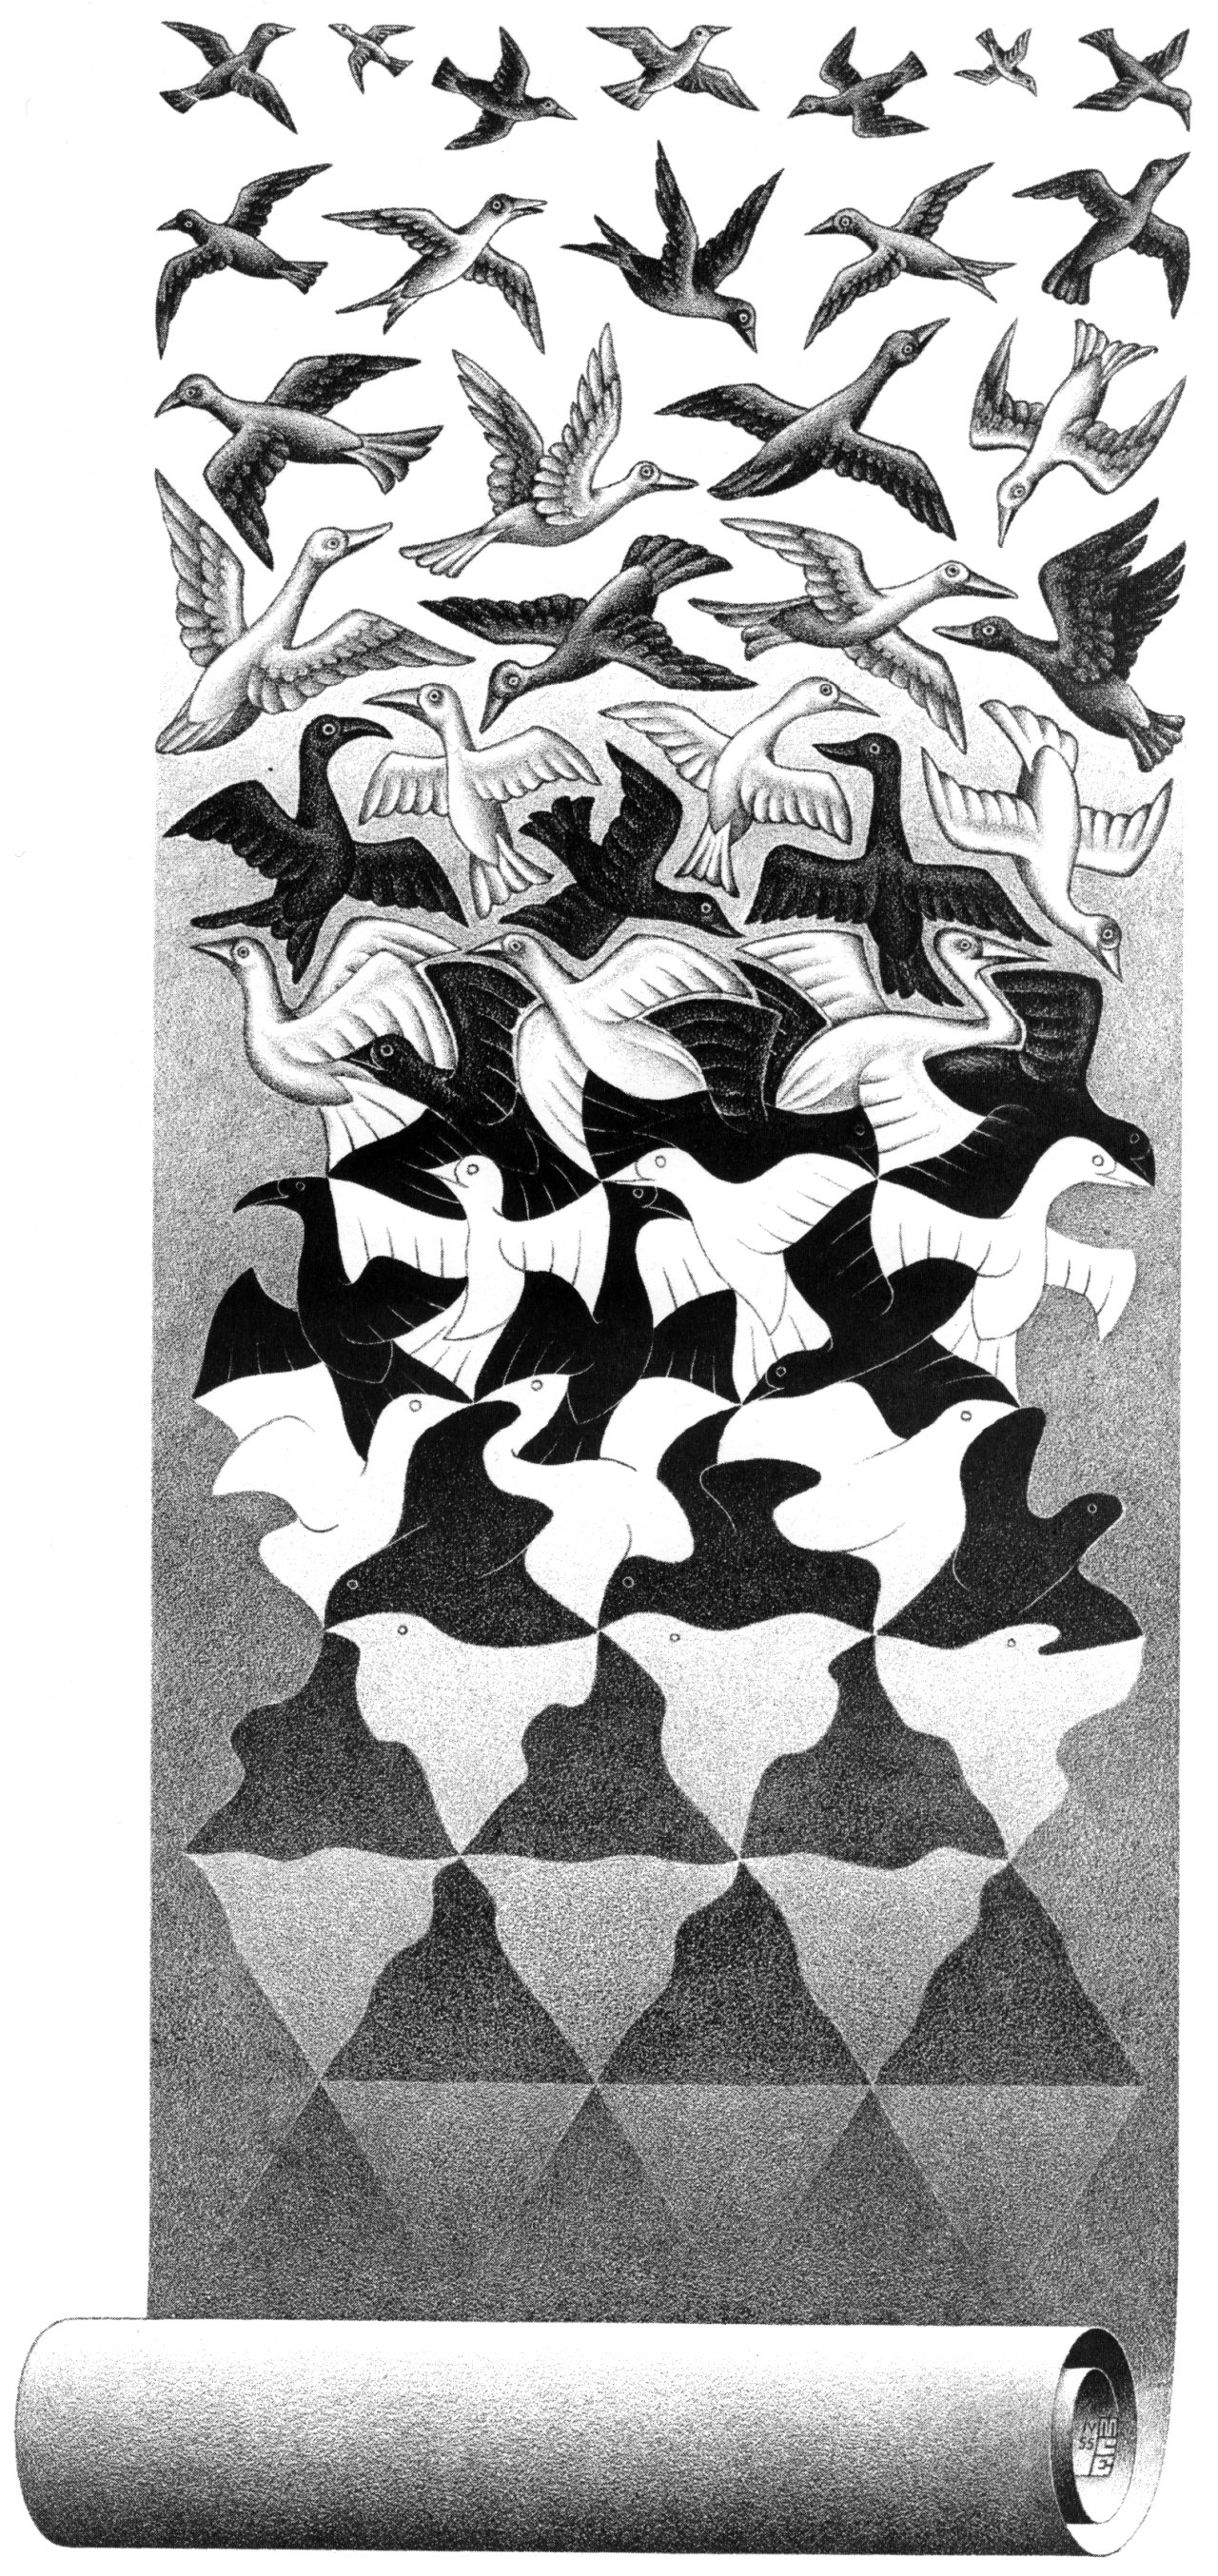
\includegraphics[scale=0.35]{img/Escher-Liberation-1955.eps}
 \captionsetup{labelformat=empty}
 \caption{Escher, Liberation, 1955}
 \label{fig:Escher-liberation}
\end{wrapfigure}

Humans gradually developed the habit of sorting things. The similar things are classified together. The methods and properties those applies to the entire class are also valid for every thing in that class. In this way, we needn't repeately solve the concrete individual problems one by one, but solve the abstract problems for a whole class. It greatly improved our ability to understand and master the world.

We generalized the abstract `folding' operation from sum and factorial for numbers. We observed their similar structures, abstract zero in sum, and one in factorial to unit element; then abstract the add in sum, and the multiplication in factorial to binary operation. As the result, we found the fold operation for numbers in a higher level. With this powerful tool, we then further solved a large sort of problems that are isomorphic to natural number, such as the Fibonacci numbers.

As another example, we also defined the abstract $foldr$ operation for list in chapter 1. With this tool, we can sum a list of numbers as $sum = foldr(0, +)$; we can also multiply them as $product = foldr(1, \times)$. In computer programming, there is a data structure called `binary search tree'. We introduced about binary tree in chapter 2. The binary search tree is a special binary tree that its elements are comparable\footnote{The meaning of comparable is abstract. If the elements are numbers, we can compare which one is bigger, if they are words, we can compare their lexicographical order.}. For any branch node, all elements in its left sub-trees are compared ahead of the element in this node; while all elements in its right sub-trees are compared behind it. Due to this kind of ordering, people also all it `sorted binary tree'. We can define insert operation for binary search tree as below:

\[
\begin{array}{rcl}
  insert(nil, x) & = & node(nil, x, nil) \\
  insert(node(l, y, r), x) & = & \left.
  \begin{cases}
  x < y\ : & node(insert(l, x), y, r) \\
  x > y\ : & node(l, y, insert(r, x))
  \end{cases} \right.
\end{array}
\label{eq:BST-insert}
\]

According to this definition, when insert element $x$ to binary search tree, if it is empty, the result is $node(nil, x, nil)$; otherwise, we need compare $x$ and the element $y$ in the branch node. If $x$ is ahead of $y$ (the `$<$' holds), then we recursively insert to the left sub-tree, else insert to the right sub-tree. Are there any similarity among the insert operation, sum, and factorial? Insertion is also binary operation, $nil$ can be considered as unit element. Then we can apply the abstract fold operation to turn a list of elements into a binary search tree:

\[
build = foldr(nil, insert)
\]

Figure \ref{fig:bst-example} shows the binary search tree generated when compute $build\ [4, 3, 1, 8, 2, 16, 10, 7, 14, 9]$.

\begin{figure}[htbp]
  \centering
  \includegraphics[scale=0.5]{img/bst-example.ps}
  \caption{The binary search tree generated from folding.}
  \label{fig:bst-example}
\end{figure}

We have similar experience when develop the concept of add. The initial addition is for specific things, like the fruits being collected, the prey being hunted. People later abstract the addition for numbers and remove the specific meanings for things. Then next we extended the understanding to numbers from integers to fractions. Although the detailed addition process is quite different, we need firstly unify the denominators, then add the nominators together, and finally reduce the fraction, people generalized the two different processes to the addition for rational numbers. We learned to think about the essence and principles of addition. Every time when people extend the concept of numbers, there is a new definition for addition. Along this way, we defined the addition for real numbers and complex numbers. We found the method established for abstract things without specific meanings has a greater scope of application. Abstract method can solve a whole kind of problems rather than the individual ones. Similar things happen in computer engineering, people developed the object-oriented method, generic type system, and dynamic type system, all these are sort of mechanisms to support abstraction.

We should always ask an important question when developing the abstract tools and generic methods. ``What is the applicable scope for the abstraction? When will the abstraction be invalid?'' It could lead to ridiculous result if ignore this. One example is about the sum of the infinite geometric series $1 + x + x^2 + x^3 + ... = 1/(1-x)$. It is so powerful that people can solved the Zeno's paradox\footnote{Here it is the Achilles and turtle paradox, which is one of the four famous paradoxes by Zeno, the ancient Greek philosopher. Achilles is a hero in ancient Greek. Zeno supposed Achilles wanted to catch up with the turtle ahead of him. When he ran to the position where the tortoise left, the tortoise had moved a short distance forward. Achilles must continue to run to that new position, but the turtle moved forward again. Repeated this process, Zeno argued that Achilles would never catch up the turtle. We'll explain Zeno's paradox in detail in Chapter 5.} with it. The mathematicians in the 17 Century substituted $x$ with -1, then got a result of $1 - 1 + 1 - 1 + ... = 1/2$. While, someone had a different idea that, $S = (1 - 1) + (1 - 1)+ ... = 0$. And there was even more different one: $S = 1 + (-1 + 1) + (-1 + 1) + ... = 1$. There were people supported the result should be 1/2, because $S = 1 - (1 - 1 + 1 - 1 + ...) = 1 -S$, solving this equation gave that $S = 1/2$. The Italian mathematician Grandi (1671 - 1742) found more surprised results. By using the infinite series:

\[
\def\arraystretch{2.2}
\begin{array}{l}
\dfrac{1}{1 + x + x^2} = 1 - x + x^3 - x^4 + x^6 - x^7 + ... \\%[5pt]
\dfrac{1}{1 + x + x^2 + x^3} = 1 - x + x^4 - x^5 + x^8 - x^9 + ... \\
...
\end{array}
\]

Let $x = 1$, Grandi found the sum of the infinite series $1 - 1 + 1 - 1 + 1 - 1 + ...$ could be 1/3, 4/1, ... Even the great mathematician Leibniz thought the result could be 0 or 1 with the same probability, therefore the `true' value should be the average 1/2. Grandi offered a new explanation that in 1710. Two brothers inherit a priceless gem from their father, whose will forbids them to sell it, so they agree that it will reside in each other's museums on alternating years. If this agreement lasts for all eternity between the brother's descendants, then the two families will each have half possession of the gem, even though it changes hands infinitely often\cite{HanXueTao16}. People kept suffering from these strange puzzles until the French mathematician Cauchy introduced the convergence concept for infinite series.

There are similar things in programming. When I implemented the natural merge sort algorithm \footnote{Natural merge sort is a sorting algorithm that permutes a list of elements in order. It firstly divides the elements into multiple groups, that every group contains the elements sorted. Then repeatedly merge these groups till all elements are ordered(\cite{LiuXinyu2017}, pp368).}, I need split the list into ordered groups, for example, split the list \texttt{[15, 9, 0, 12, 11, 7, 10, 5, 6, 13, 1, 4, 8, 3, 14, 2]} into groups of \texttt{[[15, 9, 0], [12, 11, 7], [10, 5], [6], [13, 1], [4], [8, 3], [14, 2]]}. The elements in the grouped sub-list are in descending order such as $15 > 9 > 0$. Then we can merge every two groups to get

\begin{verbatim}
[[15, 12, 11, 9, 7, 0], [10, 6, 5], [13, 4, 1], [14, 8, 3, 2]]
\end{verbatim}

Apply merge to every two groups again gives the next result

\begin{verbatim}
[[15, 12, 11, 10, 9, 7, 6, 5, 0], [14, 13, 8, 4, 3, 2, 1]]
\end{verbatim}

Then finally we can merge these two groups to get the sorted list:

\begin{verbatim}
[15, 14, 13, 12, 11, 10, 9, 8, 7, 6, 5, 4, 3, 2, 10]
\end{verbatim}

I found there is a pre-defined abstract grouping function \texttt{groupBy} in the library. It groups list with a given condition. For example \texttt{groupBy (==) "Mississippi"} gives result \texttt{["M", "i", "ss", "i", "ss", "i", "pp", "i"]}. Thus the same elements are grouped together. However, when I passed the `greater or equal' as the group condition, it generated the unexpected result. \texttt{groupBy (>=) [15, 9, 0, 12, 11, 7, 10, 5, 6, 13, 1, 4, 8, 3, 14, 2]} gives \texttt{[[15, 9, 0, 12, 11, 7, 10, 5, 6, 13, 1, 4, 8, 3, 14, 2]]}. This is because \texttt{groupBy} is realized with \texttt{span} like below:

\lstset{language=Haskell, frame=single}
\begin{lstlisting}
groupBy _  []      = []
groupBy eq (x:xs)  = (x:ys) : groupBy eq zs
    where (ys, zs) = span (eq x) xs

span _ []        = ([], [])
span p xs@(x:xs')
     | p x       = let (ys, zs) = span p xs' in (x:ys, zs)
     | otherwise = ([], xs)
\end{lstlisting}

For my example, \texttt{span} keeps checking if 15 is greater than the next element. As 15 is the biggest one in the list, therefore all the elements are grouped together. In fact, \texttt{groupBy} assumes the passed in group condition is the abstract `equality' condition, it must satisfy three properties: reflexivity, symmetry, and transitivity:

\begin{itemize}
\item reflexivity. $x = x$, any element equals to itself;
\item symmetry. if $x = y$, then $y = x$.
\item transitivity. if $x = y$, and $y = z$, then $x = z$. If two elements are identical, and one element equals to another, then the three elements are equal.
\end{itemize}

When use equality as condition to group the character list ``Mississippi'', all the three properties are satisfied, it generates the correct result. However, when pass the greater or equal ($geq$) as the abstract `equality' condition, it violates reflexivity and symmetry. That's the reason why it leads to the incorrect result.

This chapter introduces the basic abstract algebra structures. They are not only abstraction to numbers, but also the abstraction to concepts, properties, and relationships. They are the most valuable things from many great thoughts and minds. Some contents can challenge our limit of abstract thinking. It's quite common that you can't master them during the first time reading. I intended to add the stories about those great mathematicians, how they make breakthrough with unbelievable difficulties. I hope these interesting stories could encourage you keep going forward.

\section{Group}

\begin{wrapfigure}{R}{0.4\textwidth}
 \centering
 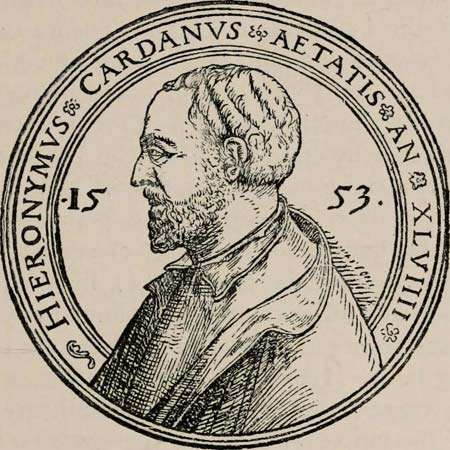
\includegraphics[scale=0.3]{img/Cardano.eps}
 \captionsetup{labelformat=empty}
 \caption{Gerolamo Cardano, 1501-1576}
 \label{fig:Cardano}
\end{wrapfigure}

\index{Gerolamo Cardano}
\index{Carl Friedrich Gauss}
\index{Fundamental theorem of algebra}

The group theory is originate from the history of equations. Equation is a powerful tool developed by ancient people. From the Rhind Mathematical Papyrus and Babylonian clay tablets, we know that the ancient Egyptians and ancient Babylonians mastered the method to solve the linear equation with one unknown and the quadratic equations. However, people didn't find the way to solve the generic cubic equations until the 16th Century. Several Italian mathematicians made great progress in solving cubic equations. Gerolamo Cardano finally published the radical solutions to generic cubic equation and quartic in his 1545 book {\em Ars Magna}. It does not only about to pursue higher and higher orders, but along with the totally new understanding about the numbers in the past thousand years. All the negative roots were discarded because we believed they were meaningless. People also thought the coefficients must be positive numbers. The equation $x^2 - 7x + 8 = 0$ is quite common today to us, but it had to be written in form of $x^2 + 8 = 7x$ to ensure the coefficients are positive. After Cardano list 20 different types of quartic equation in {\em Ars Magna}, he said there were another 67 types of quartic equation could not be given because the coefficient is either negative or zero\cite{HanXueTao2012}. It was the French mathematician François Viète who unified different forms of equations. Although most people thought the negative square root made no sense, Cardano found an interesting thing when solve the cubic equations like $x^3 = 15x +4$. His formula gives the intermediate result of $\sqrt[3]{2 + \sqrt{-121}} + \sqrt[3]{2 - \sqrt{-121}}$. Then it could next generate the three rational roots of 4, $-2 \pm \sqrt{3}$. Such problems expand our view to the irrational number, and finally, the great German mathematician Carl Friedrich Gauss developed the fundamental theorem of algebra\footnote{Gauss proved the fundamental theorem of algebra several times along his life. in 1799 at age of 22, he proved in his doctor thesis that every single-variable polynomial of degree $n$ with real coefficient has at least one complex root, thus deduced the single-variable equation of degree $n$ has and only has $n$ complex roots (counted with multiplicity for the same ones). Gauss gave another two different proofs in 1815 and 1816. In 1849, to celebrate the 50th anniversaries that Gauss received his doctor degree, he published the fourth proof and extend the coefficient to complex number.}.

\begin{figure}[htbp]
%\begin{wrapfigure}{R}{0.3\textwidth}
 \centering
 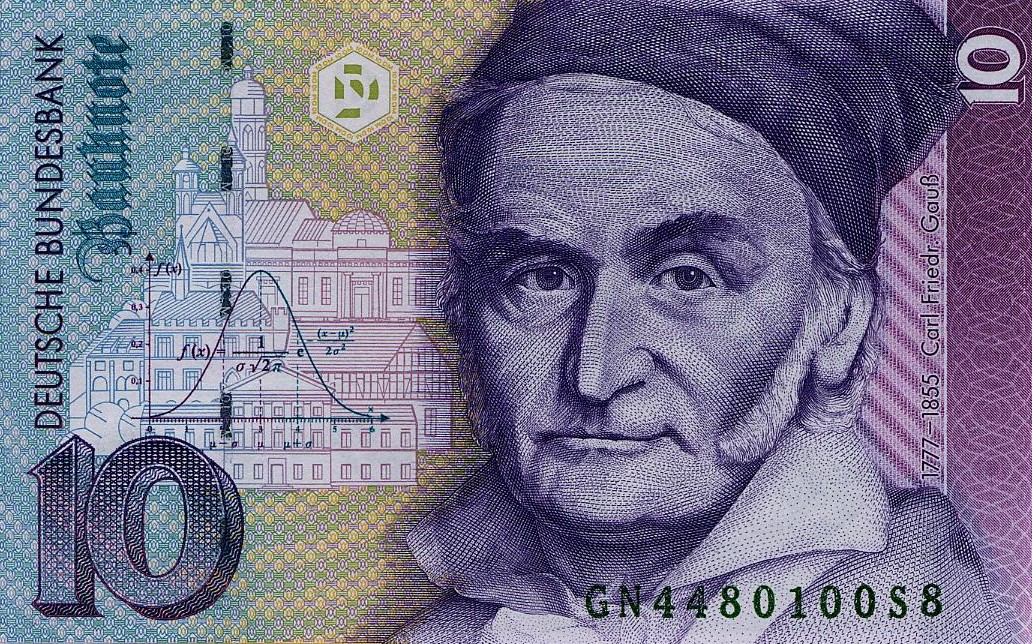
\includegraphics[scale=0.25]{img/Gaus.eps}
 \captionsetup{labelformat=empty}
 \caption{Gauss (1777-1855) in 10 Mark}
 \label{fig:Gauss}
%\end{wrapfigure}
\end{figure}

People encountered surprisingly difficulty when seek for radical solutions for generic quintic and higher order equations in the next 300 years. The breakthrough happened in the 19th Century with unexpected result. The French young Genius Évariste Galois developed a innovative idea, he was able to determine a necessary and sufficient condition for a polynomial to be savable by radicals while still in his teens\footnote{Around 1770, Joseph Louis Lagrange began the groundwork that unified the method to solve equations, he introduced the new idea to permute roots in the form of Lagrange resolvents. But he didn't consider the combination among the permutations. In 1799 The Italian mathematician Paolo Ruffini marked a major improvement, developing Lagrange's work on permutation theory. However, in general, Ruffini's proof was not considered convincing, and was discovered later incomplete. In 1824, the young Norwegian mathematician Niels Henrik Abel first completed proof demonstrating the impossibility of solving the general quintic equation in radicals. It is called `Abel–Ruffini theorem' nowadays. We know that there are radical solutions to the special quintic equation $x^5-1=0$. In what condition a polynomial is solvable in radicals? This problem was completely solved by Galois\cite{Wiki-Galois-theory}.}.

%\begin{figure}[htbp]
\begin{wrapfigure}{L}{0.4\textwidth}
 \centering
 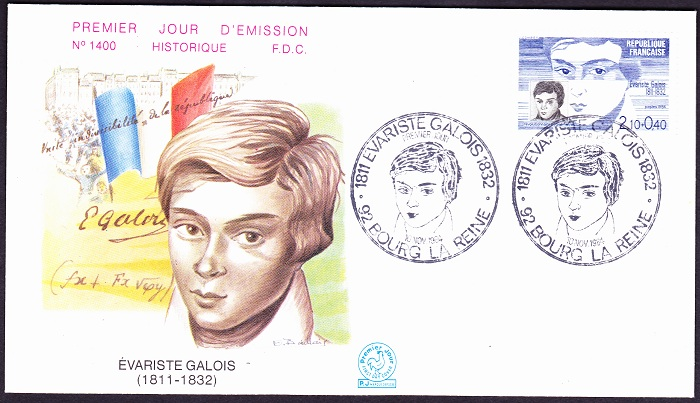
\includegraphics[scale=0.4]{img/galois.eps}
 \captionsetup{labelformat=empty}
 \caption{Galois, 1811 - 1832}
 \label{fig:Galois}
\end{wrapfigure}
%\end{figure}

\index{Galois}
It was a tragedy in Galois' short 20 years life, but his work laid the foundations of abstract algebra. Galois was born on 25 October 1811 in Paris. His mother, the daughter of a jurist, was a fluent reader of Latin and classical literature and was responsible for her son's education for his first twelve years. In 1823, he entered a prestigious school in Paris. At the age of 14, he began to take a serious interest in mathematics. He found a copy of {\em Elements} adapted by Legendre which, it is said, he read "like a novel" and mastered at the first reading. At 15, he was reading the original papers of Joseph-Louis Lagrange, which likely motivated his later work on equation theory, yet his classwork remained uninspired, and his teachers accused him of affecting ambition and originality in a negative way.

In 1828, he attempted the entrance examination for the École Polytechnique, the most prestigious institution for mathematics in France at the time, without the usual preparation in mathematics, and failed for lack of explanations on the oral examination. In that same year, he entered the École Normale, a far inferior institution for mathematical studies at that time, where he found some professors sympathetic to him.

In 1829 April, Galois' first paper, on continued fractions, was published. It was at around the same time that he began making fundamental discoveries in the theory of polynomial equations. He submitted two papers on this topic to the Academy of Sciences. But both were rejected due to some reasons\footnote{There was saying that the paper was lost by Cauchy. Actually, Cauchy refereed these papers, but refused to accept them for publication for reasons that still remain unclear. However, in spite of many claims to the contrary, it is widely held that Cauchy recognized the importance of Galois' work, and that he merely suggested combining the two papers into one in order to enter it in the competition for the Academy's Grand Prize in Mathematics. Cauchy, an eminent mathematician of the time, though with political views that were at the opposite end from Galois', considered Galois' work to be a likely winner\cite{Wiki-Galois}.}

On July 28 1829, Galois' father, a mayor of the village, committed suicide after a bitter political dispute with the village priest\cite{Wiki-Galois}. On August 3, Galois made his second and last attempt to enter the Polytechnique, and failed yet again. It is undisputed that Galois was more than qualified; however, accounts differ on why he failed. More plausible accounts state that Galois made too many logical leaps and baffled the incompetent examiner, which enraged Galois. Having been denied admission to the Polytechnique, Galois took the Baccalaureate examinations in order to enter the École Normale. He passed. His examiner in mathematics reported, ``This pupil is sometimes obscure in expressing his ideas, but he is intelligent and shows a remarkable spirit of research.''

\begin{figure}[htbp]
%\begin{wrapfigure}{L}{0.4\textwidth}
 \centering
 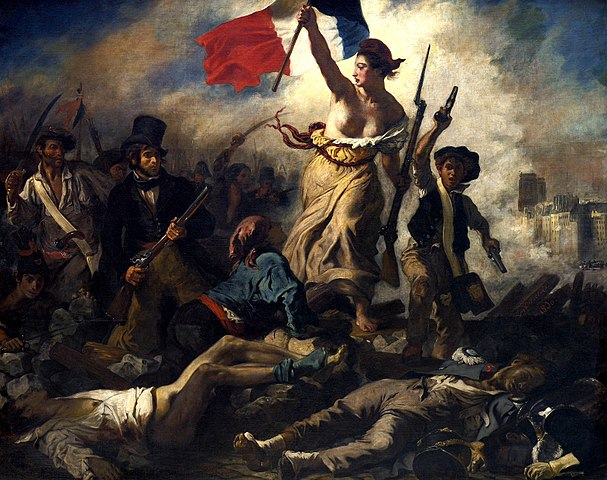
\includegraphics[scale=0.4]{img/lltp.jpg}
 \captionsetup{labelformat=empty}
 \caption{Eugène Delacroix, Liberty Leading the People, 1830, Louvre, Paris}
 \label{fig:Liberty-Leading-the-People}
%\end{wrapfigure}
\end{figure}

In February 1830, following Cauchy's suggestion Galois submitted his memoir on equation theory to the Academy's secretary Joseph Fourier, to be considered for the Grand Prix of the Academy. Unfortunately, Fourier died soon after, and the memoir was lost. The prize was awarded that year in June to Niels Henrik Abel\footnote{The young Norwegian mathematician Abel died on April 6, 1829. He made pioneering contributions in a variety of fields. His most famous single result is the first complete proof demonstrating the impossibility of solving the general quintic equation in radicals. He was also an innovator in the field of elliptic functions, discoverer of Abelian functions. He made his discoveries while living in poverty and died at the age of 26 from tuberculosis.} posthumously and also to Carl Gustav Jacob Jacobi\cite{HanXueTao2009}.

Galois lived during a time of political turmoil in France. The July Revolution broke out in France in 1830\footnote{The Bourbon monarch was restored after Napoleon's defect in Waterloo. King Charles X cleaned the soldiers who had worked for Napoleon in the army and caused dissatisfaction among the people. Continues with a series of failures in politics, economy, culture, religion, and diplomacy, Charles X signed the July Ordinances on July 25, 1830. These, among other steps, suspended the liberty of the press, dissolved the newly elected Chamber of Deputies, and excluded the commercial middle-class from future elections. It triggered the armed uprising of people, overthrew the Bourbon monarch through revolution. It ended with Louis-Philippe becoming king. Known as the July Monarchy.}. While their counterparts at the Polytechnique were making history in the streets, Galois and all the other students at the École Normale were locked in by the school's director. Galois was incensed and wrote a blistering letter criticizing the director, which he submitted to the Gazette des Écoles, signing the letter with his full name. Although the Gazette's editor omitted the signature for publication, Galois was expelled.

Galois quit school and joined the staunchly Republican artillery unit of the National Guard. He divided his time between his mathematical work and his political affiliations. Due to controversy surrounding the unit, soon after Galois became a member, on December 31, 1830, the artillery of the National Guard was disbanded out of fear that they might destabilize the government. He was arrested the on May 10, 1831, but was acquitted on June 15. On the Bastille Day (July 14), Galois was at the head of a protest, wearing the uniform of the disbanded artillery, and came heavily armed with several pistols, a rifle, and a dagger. He was again arrested. On 23 October, he was sentenced to six months in prison for illegally wearing a uniform. Early in 1831, Siméon Poisson asked him to submit his work on the theory of equations, which he did on January 17, 1831. Around July 4, 1831, Poisson declared Galois' work ``incomprehensible'', declaring that ``The argument is neither sufficiently clear nor sufficiently developed to allow us to judge its rigor\footnote{However, the rejection report ends on an encouraging note: ``We would then suggest that the author should publish the whole of his work in order to form a definitive opinion.''\cite{Wiki-Galois}}''. While Poisson's report was made before Galois' July 14 arrest, it took until October to reach Galois in prison. It is unsurprising, in the light of his character and situation at the time, that Galois reacted violently to the rejection letter, and decided to abandon publishing his papers through the Academy and instead publish them privately through his friend Auguste Chevalier. Apparently, however, Galois did not ignore Poisson's advice, as he began collecting all his mathematical manuscripts while still in prison, and continued polishing his ideas until his release on April 29, 1832.

Shortly after released from prison, Galois was involved in a obscure duel because of love. On May 29, Galois was so convinced of his impending death that he stayed up all night writing letters to his friends and composing what would become his mathematical testament, the famous letter to Auguste Chevalier outlining his ideas, and three attached manuscripts.German mathematician Hermann Weyl said of this testament, ``This letter, if judged by the novelty and profundity of ideas it contains, is perhaps the most substantial piece of writing in the whole literature of mankind.'' In these final papers, he outlined the rough edges of some work he had been doing in analysis and annotated a copy of the manuscript submitted to the Academy and other papers.

When read Galois' 7 pages testament, there are some words really sad: ``these subjects are not the only ones that I have explored... But I don't have time, and my ideas are not yet well developed in this area, which is immense...it would not be too much in my interest to make mistakes so that one suspects me of having announced theorems of which I would not have a complete proof.'' The most impressed and saddest words are: ``I don't have time'' At the end of the letter, he asked his friend to ``Ask Jacobi or Gauss publicly to give their opinion, not as to the truth, but as to the importance of these theorems. Later there will be, I hope, some people who will find it to their advantage to decipher all this mess.''\cite{Galois-1832}

\begin{figure}[htbp]
%\begin{wrapfigure}{L}{0.4\textwidth}
 \centering
 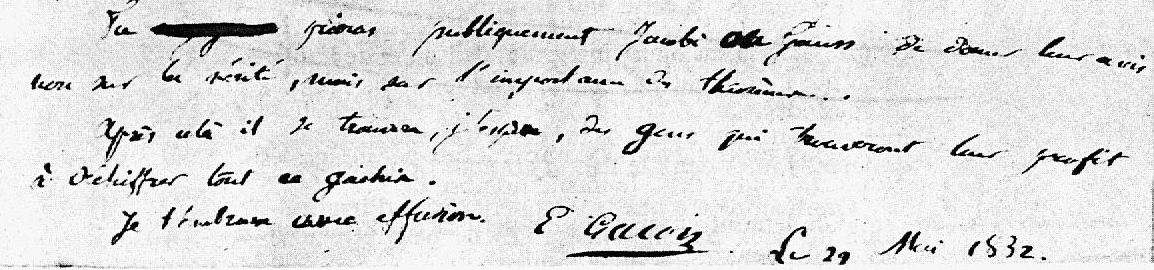
\includegraphics[scale=0.3]{img/GalSign.eps}
 \captionsetup{labelformat=empty}
 \caption{``E. Galois, le 29 mai 1832'' at the bottom of the last page in his testament.}
 \label{fig:GalSign}
%\end{wrapfigure}
\end{figure}

Early in the morning of May 30, 1832, Galois was injured badly in the duel. He was shot in the abdomen. A passing farmer found him, and sent Galois to the hospital. He died the following morning at ten o'clock, after refusing the offices of a priest. His younger brother was notified, and came to the hospital. His last words to his brother Alfred were: ``Don't cry, Alfred! I need all my courage to die at twenty!'' We don't know the exact reason behind the duel, whether it was a love tragedy or a political murder. Whatever the reason, a great talent mathematician was killed at the age of 20. He had only been studied mathematics for 5 years. Within the only 67 pages of Galois' collected works are many important ideas that have had far-reaching consequences for nearly all branches of mathematics.

Chevalier and Galois' young brother published the testament in {\em Revue encyclopedique}, but it was not noticed. It might be too brief and hard, there was almost no any impact to the mathematics in that years\footnote{The similar lessons happened to Abel as well. When he use his own money to published the paper about why quintic equation couldn't be solved by radicals in 1824, to save money, he tried all means to consolidate the paper in 6 pages. As the result, it's too brief and obscure for people to notice and understand it till Abel's death.}. Decades passed, in 1843 Liouville reviewed Galois manuscript and declared it sound. It was finally published in the October–November 1846 issue of the {\em Journal de Mathématiques Pures et Appliquées}. The most famous contribution of this manuscript was a novel proof that there is no quintic formula – that is, that fifth and higher degree equations are not generally solvable by radicals. Although Abel had already proved the impossibility of a "quintic formula" by radicals in 1824, Galois' methods led to deeper research in what is now called Galois theory. For example, one can use it to determine, for any polynomial equation, whether it has a solution by radicals. Liouville thought about this tragedy and commented it in the introduction to Galois' paper: ``Perhaps, his exaggerated desire for conciseness was the cause of this defect, and is something which one must endeavor to refrain from when dealing with the abstract and mysterious matters of pure Algebra. Clarity is, indeed, all the more necessary when one has intention of leading the reader away from the beaten roads into the desert... But at present all that has changed. Alas, Galois is no more! Let us cease carrying on with useless criticisms; let us leave its defects, and instead see its qualities... My zeal was soon rewarded. I experienced great pleasure the moment when, after having filled in the minor gaps, I recognized both the scope and precision of the method that Galois proved.''\cite{Liouville-1846}

In 1870, French mathematician Camille Jordan wrote the book {\em Traité des substitutions et des équations algébriques} based on Galois' theory\footnote{Galois' theory was notoriously difficult for his contemporaries to understand, especially to the level where they could expand on it. For example, in his 1846 commentary, Liouville completely missed the group-theoretic core of Galois' method. Joseph Alfred Serret who attended some of Liouville's talks, included Galois' theory in his 1866 (third edition) of his textbook Cours d'algèbre supérieure. Jordan was Serret's pupil. Outside France, Galois' theory remained more obscure for a longer period. It turned a century in Britain. In Germany, it was Dedekind lectured on Galois' theory at Göttingen in 1858, showing a very good understanding.}. Galois' most significant contribution to mathematics is his development of Galois theory. He realized that the algebraic solution to a polynomial equation is related to the structure of a group of permutations associated with the roots of the polynomial, the Galois group of the polynomial. It laid the foundation of group theory and lead to the development of abstract algebra and modern mathematics. As the ironic result ``Instead of the political revolution, what Galois actually triggered was the mathematics revolution\cite{StepanovRose15}.''

\subsection{Group}
\index{Group}

Let us start the journey from groups to understand what Galois landed for abstract algebra.

\begin{definition} A group is a set $G$ equipped with a binary operation ``$\cdot$'', which satisfied four axioms:

\begin{enumerate}
\item \textbf{Closure}: For all $a, b \in G$, the result of the operation $a \cdot b \in G$;
\item \textbf{Associativity}: For all $a, b, c$ in $G$, $(a \cdot b) \cdot c = a \cdot (b \cdot c)$;
\item \textbf{Identity element}: There exists an element $e$ in $G$ such that, for every element $a$ in G, the equation $a \cdot e = e \cdot a = a$ holds;
\item \textbf{Inverse element}: For each element $a \in G$, there exists an element $a^{-1}$, such that $a \cdot a^{-1} = a^{-1} \cdot a = e$, where $e$ is the identity element.
\end{enumerate}
\end{definition}

The binary operation is often called ``multiplication'', and the ``product'' $a \cdot b$ is usually written as $ab$. $e$ is the identity element. The number of elements in a group can be finite or infinite, thus the group is called finite group or infinite group. the \textbf{order} of a finite group is the number of the elements in the group. A group contains infinite many elements is said to have infinite order.

The ``multiplication'' operation of the group may not be commutative like the normal multiplication for numbers. For example, all the invertible matrix with real entities, together with the matrix multiplication form a group. However, the matrix multiplication order matters, it is not commutative. Groups for which the community equation $ab = ba$ always holds are called \textbf{abelian} groups (in honor of Abel).

To help understanding the definition of group, let us see some examples.

\begin{enumerate}
\item Integers with addition. Elements are all integers, the binary operation is addition. This is one of the most familiar groups;

\item The set of remainders of all integers divided by 5, that is $\{0, 1, 2, 3, 4\}$. The binary operation is addition then divided by 5, and take the remainder. For example $3 + 4 = 7 \bmod 5 = 2$. They form a group called addition group of integers modulo 5. Denoted as $Z_5$. We can consider it as partition the integers by taking the remainder. It is called \textbf{residue class} or residue modulo $n$;

\item The rotations of Rubik cube form a group. The elements are all cube rotations\footnote{There are 18 Rubik cube rotations. A cube move rotates one of the 6 faces, front, back, top, bottom, left, right, 90\degree, 180\degree, or -90\degree. For example, rotating the left side 90\degree, 180\degree, -90\degree can be denoted as $L$、$L^2$、$L'$\cite{Wiki-Rubik-Cube-group}. Plus the identity transform, there are total 19 elements.}, the binary operation is the composition of cube rotates, corresponding to the result of performing one cube rotate after another.

\begin{figure}[htbp]
%\begin{wrapfigure}{L}{0.4\textwidth}
 \centering
 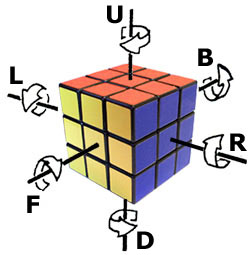
\includegraphics[scale=0.8]{img/Rubik_cube_notation.eps}
 %\captionsetup{labelformat=empty}
 \caption{There are total 18 Rubik cube rotates for the 6 faces, plus the identity transformation. These moves together with the composition operation form a group.}
 \label{fig:Rubik-cube-notation}
%\end{wrapfigure}
\end{figure}

\item For a plane, all the rotations around a fixed point form a group. The group elements are all the degrees for rotation. The group binary operation is the composition, corresponding to the result of rotating a degree after another degree.
\end{enumerate}

While the following examples are not groups:

\begin{enumerate}
\item All the integers except 0, together with multiplication do not form a group. We can't use 1 as the identity element, otherwise there will be no inverse element for 3 for example (1/3 is not integer);

\item For the same reason, remainders of modulo 5 $\{0, 1, 2, 3, 4\}$, together with multiplication modulo 5 do not form a group. However, when exclude all multiples of 5, then the set $\{1, 2, 3, 4\}$ and multiplication modulo 5 form a group. We can see this fact from the following ``multiplication table'' modulo 5:

\vspace{5mm}
  \begin{tabular}{c|cccc}
    & 1 & 2 & 3 & 4 \\
  \hline
  1 & \textbf{1} & 2 & 3 & 4 \\
  2 & 2 & 4 & \textbf{1} & 3 \\
  3 & 3 & \textbf{1} & 4 & 2 \\
  4 & 4 & 3 & 2 & \textbf{1}
  \end{tabular}
\vspace{5mm}

Therefore, 1 is the identity element, it is also the inverse element of itself; 2 and 3 are inverse element for each other; the inverse element for 4 is 4 again;

\item Although all the none zero remainders modulo 5 form a group under modulo multiplication, the none zero remainders modulo 4 do not form a group. Observe the multiplication table modulo 4:

\vspace{5mm}
  \begin{tabular}{c|cccc}
    & 1 & 2 & 3 \\
  \hline
  1 & 1 & 2 & 3 \\
  2 & 2 & \textbf{0} & 2 \\
  3 & 3 & 2 & 1 \\
  \end{tabular}
\vspace{5mm}

Note that $(2 \times 2) \bmod 4 = 0$, which is not in set $\{1, 2, 3\}$. This negative example shows that, only the remainders that are coprime to $n$ form a group under the multiplication modulo $n$. This kind of groups are called multiplicative group of integers modulo $n$. For any prime number $p$, $\{1, 2, ..., p-1\}$ forms multiplicative group modulo $p$.

\item All the rational numbers together with multiplication do not form a group. Although all rational number with form $p/q$ has a inverse element $q/p$, but there is no inverse element for 0. All the rational number exclude 0 form a group under multiplication.
\end{enumerate}

\begin{Exercise}
\Question{Do all the even number form a group under addition?}
\Question{Can we find a subset of integers, that can form a group under multiplication?}
\Question{Do all the positive real number form a group under multiplication?}
\Question{Do integers form a group under subtraction?}
\Question{Find an example of group with only two elements.}
\Question{What is the identity element for Rubik cube group? What is the inverse element for $F$?}
\end{Exercise}

\subsection{Monoid and semi-group}

The criteria to be a group is a bit strict. From the negative examples in previous section, we see some common algebraic structure can't satisfy all the axioms of the group. Sometimes we needn't inverse element. If relax the limitation, we can get the \textbf{monoid} structure.

\index{monoid}
\begin{definition}
A \textbf{monoid} is a set $S$ together with a binary operation $\cdot$, which satisfy two axioms:
\begin{enumerate}
\item \textbf{Associativity}: For any three element in $S$, the equation $(a \cdot b) \cdot c = a \cdot (b \cdot c)$ holds.
\item \textbf{Identity element}: There exists an element $e$ in $S$, such that for every element $a$ in $S$, the equations $a \cdot e = e \cdot a = e$ hold.
\end{enumerate}
\end{definition}

The monoid definition is quite similar to group except there is no axiom about inverse element. There are many negative examples for group are monoids. For example, integers under multiplication form a monoid. The identity element is 1. Monoid often appears in computer programming. We'll revisit this important algebraic structure in next chapter about category theory. Here are some more examples about monoid:

\begin{enumerate}
\item Given a character set, all finite strings with the concatenation operation form a monoid. The elements are strings; the binary operation is string concatenation; the identity element is the empty string.
\item Expand from string to list of type $A$ (List A). All lists form a monoid under the concatenation operation. The monoid elements are lists; the binary operation is the list concatenation (denoted as $\doubleplus$); the identity element is the empty list nil.

By using monoid as the algebraic structure, we can abstract both string and list as the below example program.

\begin{lstlisting}
instance Monoid (List A) where
    e = nil
    (*) = (++)
\end{lstlisting}

The folding operation to string and list, can be abstracted to the level of monoid as well\footnote{We'll introduce how to realize the abstract folding in next chapter about category theory}. The below concatenate operation for example, is defined to any monoid:

\[
concat = foldr\ e\ (*)
\]

We can concatenate list with this $concat$ operation like this:

$concat\ [[1], [2], [3], [1, 2], [1, 3], [2, 3], [1, 2, 3], [1, 3, 2]]$ gives result: [1, 2, 3, 1, 2, 1, 3, 2, 3, 1, 2, 3, 1, 3, 2].

\index{heap}
\index{skew heap}
\item Heap is a common data structure in programming. If the top element in the heap is always the minimum one, it's call the min-heap; If the top element is always the maximum one, it's called max-heap. Skew heap is a type of heap that can be realized by binary tree (\cite{LiuXinyu2017}, section 7.3).

\begin{lstlisting}
data SHeap A = nil | node (SHeap A, A, SHeap A)
\end{lstlisting}

The definition is as same as binary tree except for its name. The minimum element can be located at the root for the none empty heap. We define the merge operation for two heap as below:

\[
\begin{array}{rcl}
merge(nil, h) & = & h \\
merge(h, nil) & = & h \\
merge(h_1, h_2) & = &
  \begin{cases}
  k_1 < k_2 : & node(merge(r_1, h_2), k_1, l_1) \\
  \text{otherwise}: & node(merge(h_1, r_2), k_2, l_2)
  \end{cases}
\end{array}
\]

When merge two heaps, if one is empty, the result is the other one; if neither one is empty, we denote $h_1, h_2$ as $node(l_1, k_1, r_1)$ and $node(l_2, k_2, r_2)$ respectively. To merge them, we firstly compare their root, select the smaller one as the new root; then merge the other heap with the bigger element to one of it sub-tree. Finally, we exchange to left and right sub-trees. For example, if $k_1 < k_2$, we select $k_1$ as the new root. Then we can either merge $h_2$ to $l_1$, or merge $h_2$ to $r_1$. Without loss of generality, we merge to $r_1$. Then, we exchange the left and right sub-trees to get the final result $(k_1, merge(r_1, h_2), l_1)$. Note the binary merge operation is recursive. The set of all the skew heaps, together with the binary merge operation form a monoid. The identity element is the empty heap nil.

\index{pairing heap}
\item Heap can also be realized in multi-trees as explained in previous chapter, for example pairing heap is defined as the following (\cite{LiuXinyu2017} section 9.4):

\begin{lstlisting}
data PHeap A = nil | node (A, List (PHeap A))
\end{lstlisting}

The definition is as same as multi-tree except for its name. It is a recursive definition. A pairing heap is either empty; or a multi-tree with a root and a list of sub-trees. The minimum element is located at the root for a none empty heap. We define the merge operation for pairing heap as below:

\[
\begin{array}{rcl}
merge(nil, h) & = & h \\
merge(h, nil) & = & h \\
merge(h_1, h_2) & = &
  \begin{cases}
  k_1 < k_2 : & node(k_1, h_2 : ts_1)) \\
  \text{otherwise} : & node(k_2, h_1 : ts_2)) \\
  \end{cases}
\end{array}
\]

If either heap is empty, then the merge result is the other heap. Otherwise if neither heap is empty, we represent the two heaps $h_1$, $h_2$ as $node(k_1, ts_1)$ and $node(k_2, ts_2)$ respectively. We compare the root elements, let the bigger one as another new sub-tree of the other. The set of all the pairing heaps form a monoid under the merge operation. The identity element is the empty heap nil.

\end{enumerate}

\index{semigroup}

If relax the limitation one more step, to remove the requirement of identity element, then we get another algebraic structure, semigroup.

\begin{definition}

A semigroup is a set together with the associative binary operation.
\end{definition}

The binary operation for semigroup is associative. It means for any three elements$a$, $b$, and $c$ the equation $(ab)c = a(bc)$ holds. The constraints for semigroup is relaxed one more step. Here are some semigroup examples:

\begin{enumerate}
\item All the positive integers form a semigroup under addition, as well as under multiplication;
\item All the even numbers together with addition form a semigroup, so as under multiplication.
\end{enumerate}

As we mentioned before, people often call the binary operation for group, monoid, and semigroup as `multiplication', therefore we use the term `power' to represent applying the binary operation multiple times, for example: $x \cdot x \cdot x = x^3$. Generally, the `power' of group and monoid is defined as below recursively:

\[
x^n = \left .
  \begin{cases}
  n = 0 : & e \\
  \text{otherwise}: & x \cdot x^{n-1}
  \end{cases}
\right .
\]

For semigroup, as the identity element is not defined, $n$ must be none zero positive integer:

\[
x^n = \left .
  \begin{cases}
  n = 1 : & x \\
  \text{otherwise}: & x \cdot x^{n-1}
  \end{cases}
\right .
\]

\begin{Exercise}
\Question{The set of Boolean values \{True, False\} forms a monoid under the logic or operator $\lor$. It is called `Any' logic monoid. What is the identity element for this monoid?}
\Question{The set of Boolean values \{True, False\} forms a monoid under the logic and operator $\land$. It is called `All' logic monoid. What is the identity element for this monoid?}
\Question{For the comparable type, when compare two elements, there can be three different results. We abstract them as $\{<, =, >\}$\footnote{Some programming languages, such as C, C++, Java use negative number, zero, and positive number to represent these three results. In Haskell, they are GT, EQ, and LE respectively.}. For this set, we can define a binary operation to make it a monoid. What is the identity element for this monoid?}
\Question{Prove that the power operation for group, monoid, and semigroup is commutative: $x^mx^n = x^nx^m$}
\end{Exercise}

\subsection{The properties of group}

One powerful idea in abstract algebra is that, we can focus on the inner patterns of the abstract structures and their relationships without the need to care about the concrete object and its meaning. The pattern and the revealed the insight are applicable to all the object by the nature of abstraction. When we understand the generic properties of group, if the elements represent the points, lines, and surfaces, then we gain the properties of geometry; if the elements represent Rubik cube rotations, then we gain the properties of Rubik cube transformation; if the elements represent some data structure in programming, we gain the properties of the algorithm on top of that data structure. We introduce some important properties for groups in this section.

\begin{theorem}
There is one and only one identity element for any group.
\end{theorem}

\begin{proof}
Suppose there is another identity element $e'$, for all element $a$, the equations $e'a = ae' = a$ hold. Substitute $a$ to $e$, we have $e = ee'= e'$. Thus proved the uniqueness of the identity element.
\end{proof}

For any group, not only the identity element is unique, but the inverse element for every element is also unique.

\begin{theorem}
The unique existence of inverse element. For all element $a$, there is one and only one $a^{-1}$ that satisfies $aa^{-1} = a^{-1}a = e$. We call $a^{-1}$ the inverse element of $a$.
\end{theorem}

\begin{proof}
We know the existence of inverse element from the group axiom of identity element. So we only need proof the uniqueness. Suppose there exists another element $b$, that also satisfies $ab = ba = e$. We multiply $a^{-1}$ to the equation from right to get:

\[
\begin{array}{rll}
aba^{-1} & = baa^{-1} = ea^{-1} & \\
& \Rightarrow be = a^{-1} & \text{Apply associative law to the 2nd term} \\
& \Rightarrow b = a^{-1} & \text{Uniqueness of the inverse element}
\end{array}
\]
\end{proof}

\begin{figure}[htbp]
%\begin{wrapfigure}{L}{0.4\textwidth}
 \centering
 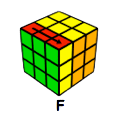
\includegraphics[scale=1.0]{img/Rubik-cube-F.eps}
 %\captionsetup{labelformat=empty}
 \caption{The F move of Rubik cube, repeat rotating F 4 times returns to the original state.}
 \label{fig:Rubik-cube-F}
%\end{wrapfigure}
\end{figure}

\index{The order of the group element}
We defined the order for group before. For group element, we can define order as well. For element $a$, the minimum positive integer $m$ that satisfies $a^m = e$ is called the order of $a$. If such $m$ does not exist, we say the order of $a$ is infinite. Using the Rubik cube group for example, if we repeat F rotation 4 times, the cube returns to its original state. Therefore, the order for F is 4. Because repeat $F'$ twice returns the original state, the order is 2. Another example is the integer multiplicative group modulo 5. All elements except 1, the power of 4 modulo 5 are 1, all their orders are 4. Actually, we have the following interesting theorem:

\begin{theorem}
For any finite group, all elements have finite order.
\end{theorem}

\begin{proof}
Denote the order for a given finite group $G$ as $n$. For any element $a$, we can construct a set $\{a, a^2, ..., a^{n+1}\}$. There are $n + 1$ elements in this set, however, the order of the group is $n$. According to the principle of pigeon hole. There are at least two equal elements. Denote such two equal elements as $a^i$ and $a^j$, where $0 < i < j \leq n + 1$ without loss of generality. We have:

\[
\begin{array}{rcll}
a^ja^{-i} & = & a^{-i}a{i} & \text{由} a^i = a^j \\
a^ja^{-i} & = & e & \text{$a^i$ is inverse to $a^{-i}$} \\
a^{j-i} & = & e & \text{the order of $a$ is}\ j - i
\end{array}
\]
Thus the order of $a$, $j - i$ is finite.
\end{proof}

We use the term `isomorphism' in chapter 1 to describe things that have the same inner structure. It's time to give the strict definition for homomorphism and isomorphism. Suppose there is a mapping (morphism) $f$ from set $A$ to set $B$. $a$ and $b$ are two elements in $A$, their images in $B$ are $f(a)$ and $f(b)$ respectively. Let's consider an element $a \cdot b$, which is result of the binary closed operation defined in $A$. Under the map (morphism) $f$, its image in $B$ is $f(a \cdot b)$. If for the binary closed operation defined in $B$, the following equation always holds:

\[
f(a) \cdot f(b) = f(a \cdot b)
\]

\begin{figure}[htbp]
\centering
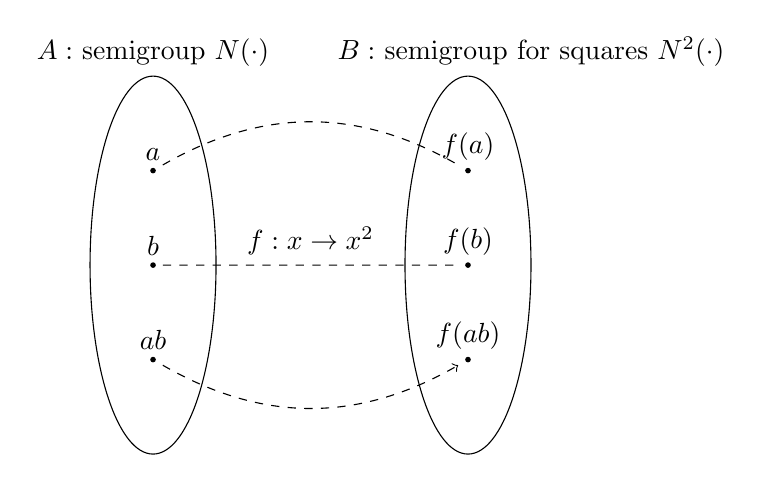
\begin{tikzpicture}[scale=0.8]
\draw (0, 0) circle[x radius=1cm, y radius=3cm]
      (5, 0) circle[x radius=1cm, y radius=3cm];
\path (0, 3) node[above] {$A:$ semigroup $N(\cdot)$}
      (6, 3) node[above] {$B:$ semigroup for squares $N^2(\cdot)$};
\path (0, 0) node (b) {}
      (5, 0) node (fb) {}
      (0, 1.5) node (a) {}
      (5, 1.5) node (fa) {}
      (0, -1.5) node (c) {}
      (5, -1.5) node (fc) {};
\filldraw (0, 0) circle (1pt) node[above] {$b$}
      (5, 0) circle (1pt) node[above] {$f(b)$}
      (0, 1.5) circle (1pt) node[above] {$a$}
      (5, 1.5) circle (1pt) node[above] {$f(a)$}
      (0, -1.5) circle (1pt) node[above] {$ab$}
      (5, -1.5) circle (1pt) node[above] {$f(ab)$};
\draw[dashed, ->] (b) to node [above] {$f: x \to x^2$} (fb)
      (a) to [bend left] (fa)
      (c) to [bend right] (fc);
\end{tikzpicture}
\[
\begin{array}{rl}
a = 2 & f(a) = 4 \\
b = 3 & f(b) = 9 \\
ab = 6 & f(ab) = f(a)f(b) = 36
\end{array}
\]
\caption{Isomorphism}
\label{fig:isomorphism}
\end{figure}

\index{homomorphism}
We say $f$ is a \textbf{homomorphism} from $A$ to $B$. If $f$ is a surjection, known as `onto', which means all elements $b$ in $B$, has the corresponding $a$ in A, that $f(a) = b$, then $f$ is called surjective homomorphism. For example, consider a test function $odd: Z \to Bool$, it accepts a integer number, if the number is odd, then it returns True, otherwise returns False. All integers form a group under addition, while the Boolean value set $\{True, False\}$ also forms a group under logic exclusive or operation. We can verify that:

\begin{enumerate}
\item Both $a$ and $b$ are odd numbers. $odd(a)$ and $odd(b)$ are both True. Their sum is even, $odd(a+b)$ is False. Equation $odd(a) \oplus odd(b) = odd(a+b)$ holds;
\item Both $a$ and $b$ are even numbers. $odd(a)$ and $odd(b)$ are both False. Their sum is also even, $odd(a+b)$ is False. Equation $odd(a) \oplus odd(b) = odd(a+b)$ holds;
\item $a$ and $b$ one is odd, the other is even; $odd(a)$ and $odd(b)$ one is True, the other is False. Their sum is odd, $odd(a+b)$ is True. Equation $odd(a) \oplus odd(b) = odd(a+b)$ holds.
\end{enumerate}

\index{isomorphism}
\index{automorphism}
If $f$ is not only a surjection, but also a injection (there are no any two different elements map to the same image), then it's one-to-one mapping. We call $f$ is the \textbf{isomorphism} from $A$ to $B$. Denote as $A \cong B$. Isomorphism is a very powerful relationship. It does not only apply to two groups, but also applicable to semigroups, monoids and other algebraic structures. As shown in figure \ref{fig:isomorphism}. If $A$ is isomorphic to $B$, from abstracted view, they are essentially same things with different names. If there is a algebraic property in $A$, then there is exactly a same property in $B$ as well(\cite{ZhangHeRui1978} pp.25). The special isomorphism from $A$ to $A$ is called \textbf{automorphism} of $A$. For example, the group of integers with addition has a automorphism under the negate operation.

\begin{figure}[htbp]
\centering
\begin{tikzpicture}
\path (0, 0) node[below] {cat}
      (0, 2) node[above] {sheep}
      (-2, 2) node[above] {dog}
      (-2, 0) node[below] {cow};
\filldraw (0, 0) circle (4pt) node (cat) {} --
   (0, 2) circle (4pt) node (sheep) {} --
   (-2, 2) circle (4pt) node (dog) {} --
   (-2, 0) circle (4pt) node (cow) {};
\draw (dog) -- (cat) -- (cow);

\filldraw[fill=gray, draw=black, pattern=north west lines]
    (3, 0) circle (4pt) node (collar) {} --
    (5.6, 0) circle (4pt) node (bell) {} --
    (4.3, 2.3) circle (4pt) node (milk) {} -- (collar) --
    (4.3, 1) circle (4pt) node (wool) {} -- (bell);
\path (3, 0) node[below] {collar}
      (5.6, 0) node[below] {bell}
      (4.3, 2.3) node[above] {milk}
      (4.3, 1) node[below] {wool};

\draw[dashed, ->] (dog) .. controls (-2.5, 1.5) .. (collar)
    (sheep) to[bend left] (wool)
    (cat) to[bend right] (bell)
    (cow) .. controls (-3, 3) ..(milk);
\end{tikzpicture}
\[
\begin{array}{rl}
f(dog) = collar & f(cat) = bell \\
f(sheep) = wool & f(cow) = milk
\end{array}
\]
\caption{The graph isomorphism has different meaning. The two different graph has the same structure.}
\label{fig:graph-isomorphism}
\end{figure}

People often use the familiar concrete example to understand abstract algebraic structure. For groups, most time, we think about integers with addition, how those concepts, properties of group will be for integers? But such approach may give us illusion that the element of group is kind of entity, like numbers; and the binary operation is more like the common addition or multiplication that can be commutative. We'll introduce an `exceptional' example, the transformation group. On one hand, it is not Abelian, the binary operation is not commutative; on the other hand, the its group elements are not numbers, but transformations.

Transformation is a map from set $A$ to $A$ itself. Denoted as $\tau : A \to A$. It maps element $a$ in $A$ to $\tau(a)$. That is $a \to \tau(a)$. There are varies transformations for a set. The following is all the transformations for Boolean set, we denote true as $T$, false as $F$.

\[
\begin{array}{rll}
\tau_1 : & T \to T, & F \to T \\
\tau_2 : & T \to F, & F \to F \\
\tau_3 : & T \to T, & F \to F \\
\tau_4 : & T \to F, & F \to T
\end{array}
\]

Among them, $\tau_3$ and $\tau_4$ are one to one transformations. For a given set $A$, all its transformations form a new set:

\[
S = \{\tau, \lambda, \mu, ...\}
\]

Let's next define a binary operation for $S$, and call it as multiplication. For convenient purpose, we express $\tau(a)$ as this way:

\[
\tau: a \to a^\tau = \tau(a)
\]

Note that $a^\tau$ does not mean the $\tau$ power of $a$. It is only a notation means transformation. Observe two elements $\tau$ and $\lambda$ in $S$.

\[
\tau: a \to a^\tau,  \lambda: a \to a^\lambda
\]

We can find that $a \to (a^\tau)^\lambda = \lambda(\tau(a))$ is also a transformation for $A$. We define it is the product of $\tau$ and $\lambda$.

\[
\tau\lambda: a \to (a^\tau)^\lambda = a^{\tau\lambda}
\]

Such multiplication is actually composition operation of two transformations. Please select some from the list of Boolean transformations to verify their product. The multiplication is actually associative, since:

\[
\begin{array}{rl}
\tau(\lambda\mu): & a \to (a^\tau)^{\lambda\mu} = ((a^\tau)^\lambda)^\mu \\
(\tau\lambda)\mu: & a \to (a^{\tau\lambda})^\mu = ((a^\tau)^\lambda)^\mu
\end{array}
\]

We benefit from the power of power expression. We can't say too much about a powerful notation system in the history of math. Euler, Leibniz are all masters of inventing great symbols. For the above multiplication we defined, the identity element in $S$ is the identity transformation of $A$, which maps every element to itself, $\epsilon: a \to a$. We can verify that:

\[
\begin{array}{rl}
\epsilon\tau: & a \to (a^\epsilon)^\tau = a^\tau \\
\tau\epsilon: & a \to (a^\tau)^\epsilon = a^\tau
\end{array}
\]

Therefore $\epsilon\tau = \tau\epsilon = \tau$. With this multiplication operation, set $S$ almost form a group. We say it `almost', it eventually can not form a group. This is because for a given transformation $\tau$, there is not necessarily an inverse element. For example the $\tau_1$ in the Boolean set, it maps any Boolean value to true. None of the 4 transformations can change $\tau_1$ back. Thus there is no reverse element for $\tau_1$.

Although $S$ can not form a group, interestingly, its subgroup $G$ can. In fact, as long as $G$ contains the one-to-one transformation of $A$, then it form a group under the multiplication operation.

\index{transformation group}

For set $A$, the set of one to one transformations of $A$ together with the composite operation (defined above as multiplication) form a \textbf{transformation group} of $A$. We have the below important theorem:

\begin{theorem}
All the one to one transformations of set $A$ form a transformation group $G$.
\end{theorem}

Transformation groups are not necessarily Abelian. It's easy to find negative examples. Consider the shift transformation $\tau_1$ which moves the origin from (0, 0) to (1, 0), and the rotation transformation $\tau_2$ which rotate around the origin by $\pi/2$. We have:

\[
\begin{array}{rl}
\tau_1\tau_2: & (0, 0) \to (0, 1) \\
\tau_2\tau_1: & (0, 0) \to (1, 0)
\end{array}
\]

\begin{figure}[htbp]
\centering
\begin{tikzpicture}[scale=1]
\draw[->] (-0.5, 0) -- (2, 0) node[right] (x axis) {$x$};
\draw[->] (0, -1.5) -- (0, 1.5) node[above] (y axis) {$y$};
\path (0, -1) node[left] {$a$}
      (1, -1) node[right] {$b$}
      (1, 1) node[above] {$c$};
\filldraw (0, -1) circle(1pt) node (a) {}
          (1, -1) circle(1pt) node (b) {}
          (1, 1) circle(1pt) node (c) {};
\draw[dashed, ->] (a) -- (b);
\draw[dashed, ->] (b) .. controls (1.4, 0) .. (c);
\draw (0, 0) -- (1.2, -1.2)
      (0, 0) -- (1.2, 1.2)
      (1, 0) arc (0:45:1)
      (1, 0) arc (0:-45:1);

\draw[->] (3.5, 0) -- (6.5, 0) node[right] (x axisr) {$x$};
\draw[->] (4, -1.5) -- (4, 1.5) node[above] (y axisr) {$y$};
\filldraw (4, -1) circle (1pt) node[left] (a1) {$a$}
      (5, 0) circle (1pt) node[above] (b1) {$b'$}
      (6, 0) circle (1pt) node[above] (c1) {$c'$};
\draw[dashed, ->] (a1) .. controls (4.7, -0.7) .. (b1);
\draw[dashed, ->] (b1) -- (c1);
\draw (5, 0) arc (0:-90:0.8);
\end{tikzpicture}
\caption{The transform order matters. The results are different}
\label{fig:transform-not-abelian}
\end{figure}

Therefore, this transformation group is not Abelian. Transform groups are important and have wide applications. We have a strong fact:

\begin{theorem}
Every group is isomorphic to a transformation group.
\end{theorem}

% TODO:附录
We skip the proof. This theorem tells us, for any abstract group, we can find a concrete instance as a transformation group. In other words, we needn't concern about finding an abstract group in the future, which is totally a castle in the air(\cite{ZhangHeRui1978} pp49).

\begin{Exercise}
\Question{Is the odd even test function homomorphic between the integer addition group $(Z,+)$ and the Boolean logic and group $(Bool, \land)$? What about the group of integers without zero under multiplication?}
\Question{Suppose two groups $G$ and $G'$ are homomorphic. In $G$, the element $a \to a'$. Is the order of $a$ same as the order of $a'$?}
\Question{Prove that the identity element for transformation group must be identity transformation.}
\end{Exercise}

\subsection{Permutation group}
\label{permutation group}
\label{symmetric group}

In this section, we introduce permutation group. It is the permutation group that Galois used to determine if a given equation is solvable by radicals. Permutation group is a special transformation group. Let's first define what is permutation. A \textbf{permutation} is a one to one transformation for a finite set. The permutations of a finite set form a \textbf{permutation group} under the composite operation. As the name indicates, it permutes elements in the set. Further, the group of {\em all} permutations of a set of $n$ elements is the \textbf{symmetric group} of degree $n$, denoted as $S_n$.

We know from the permutation theory learned in high school, there are $n!$ different permutations for $n$ elements. Therefore, the symmetric group of degree $n$ has the order of $n!$. A permutation maps element $a_i$ in the set to $a_{k_i}$, where $i = 1, 2, ..., n$. The permutation can be determined by $n$ pairs of $(1, k_1), (2, k_2), ..., (n, k_n)$. We can express the permutation as:

\[
\begin{pmatrix}
1 & 2 & ... & n \\
k_1 & k_2 & ... & k_n
\end{pmatrix}
\]

For example

\[
\begin{pmatrix}
1 & 2 & 3 & 4 & 5 \\
2 & 5 & 4 & 3 & 1
\end{pmatrix}
\]

It represents a permutation. Since the first row is always in the form $1, 2, ..., n$, we can further simplify the permutation to $(2, 5, 4, 3, 1)$. It means this permutation change the 2nd element to the 1st; change the 5th element to the 2nd and so on. We can use this notation to list all permutations for a set contains 3 elements, which is the elements for group $S_3$:

\[
(1, 2, 3), (1, 3, 2), (2, 1, 3), (2, 3, 1), (3, 1, 2), (3, 2, 1)
\]

When do the multiplication, which is composition essentially, we can determine the element for every position as this. For the $i$-th position, first check what the new position should be in the first permutation, for example $j$; then check where $j$ should be mapped to in the second permutation, for example $k$. Therefore, the final position as the result of the multiplication is $k$. Let's pick two elements from group $S_3$, to examine if it is Abelian:

\[
\begin{array}{l}
(1, 3, 2) (2, 1, 3) = (2, 3, 1) \\
(2, 1, 3) (1, 3, 2) = (3, 1, 2)
\end{array}
\]

They are different results, $S_3$ is not Abelian. Actually, it is the smallest finite none Abelian group. A finite none Abelian group contains at least 6 elements. Observe the permutation for 5 elements $(2, 3, 1, 4, 5)$, only the first three ones change, while the rest two keep same. The changes for the first three elements have a pattern: $2 \to 1$, $3 \to 2$, $1 \to 3$. They are cyclic.

\begin{figure}[htbp]
\centering
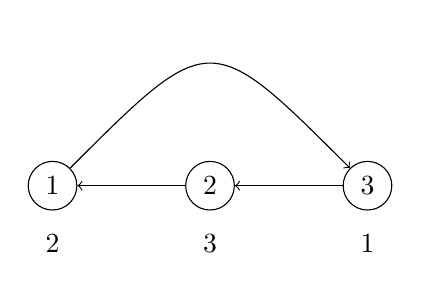
\begin{tikzpicture}[scale=1]
\path (0, 0) node[circle, draw] (1) {1}
      (2, 0) node[circle, draw] (2) {2}
      (4, 0) node[circle, draw] (3) {3};
\draw[<-] (1) edge (2)
          (2) edge (3)
          (3) .. controls (2, 2) .. (1);
\path (0, -0.5) node[below] {2}
      (2, -0.5) node[below] {3}
      (4, -0.5) node[below] {1};
\end{tikzpicture}
\caption{Permutation $(2\ 3\ 1)$ is cyclic}
\label{fig:cycle-permutation}
\end{figure}

With this pattern, we can simplify the permutation notation from $(2, 3, 1, 4, 5)$ to $(2\ 3\ 1)$. Note there is no comma between elements, and we treat $(1\ 2\ 3)$, $(2\ 3\ 1)$, and $(3\ 1\ 2)$ represent the same 3-cyclic permutation\footnote{There are people use $(231)$ notation without any spaces as deliminator. However, when there are over 10 elements, it cause ambiguity. As it can also be $(23\ 1)$.}. Formally, we define $k$-cyclic permutation $(i_{j_1} i_{j_2} ... i_{j_k})$. It maps the next element to its previous position, and send the first element to the last to form the cycle:

\[
i_{j_2} \to i_{j_1}, i_{j_3} \to i_{j_2}, ..., i_{j_1} \to i_{j_k}
\]

The elements in $k$-cyclic permutation are not necessary adjacent, for example $(3\ 9\ 4)$, nor in a fixed order, for example $(2\ 4\ 1\ 3)$. If there are only two element in the circle, like $(i\ j)$, we call it transposition. Identity transformation is the special case, for example $(1, 2, 3, 4, 5)$, we denote it as $\epsilon = (1)$, and let:

\[
\epsilon = (1) = (2) = ... = (n)
\]

Observe the permutation $(2, 1, 4, 5, 3)$, it contains two cycles, one is the 2-cyclic permutation $(1\ 2)$, the other is 3-cyclic permutation $(3\ 4\ 5)$. We can use the permutation multiplication to express this fact:

\[
(2, 1, 4, 5, 3) = (1\ 2)(3\ 4\ 5)
\]

In fact, every permutation $\pi$ for $n$ elements can be expressed with some mutual exclusive (without any common numbers) cyclic permutations. This approach brings us a useful advantage, although permutations are not commutative in common case, as $k$-cyclic permutations don't share same numbers, they are commutative. For example $(1\ 2)(3\ 4\ 5) = (3\ 4\ 5)(1\ 2)$.

The following list express all the permutations in $S_3$ in this way:

\[
(1),
(1\ 2), (1\ 3), (2\ 3),
(1\ 2\ 3), (1\ 3\ 2)
\]

Given a permutation $(k_1, k_2, ..., k_n)$, how to express it as the product of cyclic forms? We can do it with such prescription. From left to right compare every position with the number in the permutation, if $k_i$ equals $i$, it means the element has already in the right position; otherwise open a pair of parentheses, write down the number in position $k_i$ in the parentheses, let say it is $k_j$, then check the position $k_j$ with $j$, if they are not equal, write in the parentheses. Repeat this step till we found some element form a circle to the starting point. At this time point, we close the parentheses of this cycle. After that, we go on checking from left to right till all the elements are processed (\cite{Armstrong1988}, pp27). If for all position, we have $k_i$ equals to $i$, then we write down $(1)$ to present the identity permutation. It very convenient to realize this process in programming way. Below is the algorithm for it and an example source code in a real programming language.

\begin{algorithmic}
\Function{k-cycles}{$\pi$}
  \State $r \gets []$
  \For{$i \gets 1$ to $|\pi|$}
    \State $p \gets []$
    \While{$i \neq \pi[i]$}
      \State $p \gets \pi[i]:p$
      \State Exchange $\pi[i] \leftrightarrow \pi[\pi[i]]$
    \EndWhile
    \If{$p \neq []$}
      \State $r \gets r:(\pi[i]:reverse(p))$
    \EndIf
  \EndFor
  \If{$r \neq []$}
    \State \Return r
  \Else
    \State \Return $[[1]]$ \Comment{Identity permutation}
  \EndIf
\EndFunction
\end{algorithmic}

Express any permutation as product of $k$-cycle notation:

\lstset{language=Python}
\begin{lstlisting}
def kcycles(a):
    r = []
    n = len(a)
    for i in range(n):
        p = []
        while i + 1 != a[i]:
            p.append(a[i])
            j = a[i] - 1
            a[i], a[j] = a[j], a[i]
        if p != []:
            r.append([a[i]] + p)
    return r if r != [] else [[1]]
\end{lstlisting}

From the theorem in previous section, we further have:

\begin{theorem}
Every finite group is isomorphic to a permutation group.
\end{theorem}

For any finite group, like the solutions of a equation, we can study it with the permutation group, as the permutation group is easy to manipulate. This is exactly how Galois solve the problem to determine if the equation is solvable by radicals.

\begin{Exercise}
\Question{List all the elements in $S_4$.}
\Question{Express all the elements in $S_3$ as the product of cyclic forms.}
\Question{Write a program to convert the product of $k$-cycles back to permutation.}
\end{Exercise}

\subsection{Cyclic group}

\index{cyclic group}
Among all the groups, the cyclic group is the easiest. It's the kind of groups that completely understood as of today. Is it possible that all the elements in a group $G$ are power of a given element? Such group does exist. Consider the integer multiplicative group modulo 5 without 0 for example. It contains 4 elements $\{1, 2, 3, 4\}$. If list all the powers of 2 modulo 5, we have the following result:

\[
\begin{array}{l}
2^1 \bmod 5 = 2 \\
2^2 \bmod 5 = 4 \\
2^3 \bmod 5 = 3 \\
2^4 \bmod 5 = 1
\end{array}
\]

Thus the powers of 2 generate all the elements in this group. We define:

\begin{definition}
If all the elements in a group $G$ are the power of a fixed element $a$, we say $G$ is a \textbf{cyclic group}. In other words $G$ is generated by element $a$, denoted as:

\[
G = (a)
\]

We call $a$ the generator of group $G$.
\end{definition}

Let us see two important examples of cyclic group:

\begin{example}
The additive group of integers. All integers are `power' of 1. Here the binary operation is addition, therefore, power means keep adding 1. For any positive integer $m$:

\[
\begin{array}{rcll}
1^m & = & 1 \cdot 1 \cdot 1 \cdot ... \cdot 1 & \text{$m$ power of} \\
    & = & 1 + 1 + ... + 1 & \text{+ is the multiplicative operation for $G(Z, +)$} \\
    & = & m &
\end{array}
\]

In additive group of integers, the inverse element of 1 is -1. This is because 1 + (-1) = 0, and 0 is the identity element. For any negative integer $-m$:

\[
\begin{array}{rcll}
1^{-m} & = (-1)^m & \text{inverse element} & \\
(-1)^m & = & (-1) \cdot (-1) \cdot (-1) \cdot ... \cdot (-1) & \text{$m$次} \\
       & = & -1 + (-1) + ... + (-1) & \text{+ is the multiplicative operation for $G(Z, +)$} \\
       & = & -m &
\end{array}
\]

As 0 is the identity element, we define $0 = 1^0$. Summarize all these three cases, we have $Z = (1)$.
\end{example}

The additive group of integers is an example of infinite cyclic group. Let us see an example of finite cyclic group.

\begin{example}
Consider integers residue modulo $n$. For integer $a$, we use notation $[a]$ to represent the residue $a$ belongs to. Define the binary operation as the addition modulo $n$.

\[
[a] + [b] = [a + b]
\]

For instance, when compute $[3] + [4]$ modulo 5, the result is $7 \bmod 5 = [2]$. It's easy to verify this binary operation satisfies the associative law. The identity element is [0], and all elements have inverse. We cal l this group additive group of integer residues modulo $n$. The group elements are [0], [1], ..., [$n$-1]. It is a cyclic group because every element [$i$] can be expressed as $i$ power of [1].

\[
[i] = [1] + [1] + ... + [1] \quad \text{Total $i$ times}
\]
\end{example}

We intentionally choose these two examples. In fact, we've already understood all the cyclic groups through these two examples! This is because of the following theorem:

\begin{theorem}
If $G$ is a cyclic group generated by element $a$, then the algebraic structure of $G$ is completely determined by order of $a$:
\begin{itemize}
\item If the order of $a$ is infinite, then $G$ is isomorphic to the additive group of integers;
\item If the order of $a$ is $n$, then $G$ is isomorphic to the additive group of integer residues modulo $n$.
\end{itemize}
\end{theorem}

\begin{proof}
If the order of $a$ is infinite, we have $a^h = a^k$ if and only if $h = k$. Otherwise, if $h \neq k$, let $h > k$ without loss of generality, we have $a^{h - k} = e$, which conflicts with the condition that the order of $a$ is infinite. Therefore, we can construct a one to one map:

\[
f: a^k \to k
\]

This map is isomorphic between the cyclic group $G = (a)$ and the additive group of integers $Z$. That is $a^ha^k \to h + k$.

If the order of $a$ is integer $n$, which means $a^n = e$. Then $a^h = a^k$ if and only if $h \equiv k \mod n$. We can construct another one to one map:

\[
f: a^k \to [k]
\]

This map is isomorphic between the cyclic group $G = (a)$ and the additive group of integer residues modulo $n$. That is:

\[
a^ha^k = a^{h + k} \to [h + k] = [h] + [k]
\]
\end{proof}

Therefore, from the abstraction perspective, there is only one group that the order of generator is infinite, and there is only one group that the order of generator is a given positive integer. We clearly understand the algebraic structure of these cyclic groups:

\begin{itemize}
\item The order of $a$ is infinite
  \begin{itemize}
  \item Group elements: ..., $a^{-2}, a^{-1}, a^0, a^1, a^2$, ...
  \item Binary operation: $a^ha^k = a^{h + k}$
  \end{itemize}
\item The order of $a$ is $n$
  \begin{itemize}
  \item Group elements: $a^0, a^1, a^2, ..., a^{n-1}$
  \item Binary operation: $a^ha^k = a^{(h + k) \bmod n}$
  \end{itemize}
\end{itemize}

\begin{Exercise}
\Question{Proof that cyclic groups are Abelian.}
\end{Exercise}

\subsection{Subgroup}
\index{subgroup}

The next important concept is subgroup. It can help us to understand the properties of a group through its subset.

\begin{definition}
For a given group $G$, a subset $H$ of $G$ is called \textbf{subgroup} if $H$ forms a group under the multiplication of $G$.
\end{definition}

For any group $G$, there are at least two subgroups. One is $G$ itself, the other is a singleton set only contains the identity element $\{e\}$. They are are called trivial subgroups. Taking the additive group of integers for example, all the even numbers under addition form a subgroup, while the odd numbers do not form a subgroup (do you know why?). Here is another example, for the permutation group $S_3$, consider its subset $H = \{(1), (1\ 2)\}$. $H$ form a subgroup under the composite operation. We can verify it as the following:

\begin{enumerate}
\item Close under multiplication: $(1)(1) = (1)$, $(1)(1\ 2) = (1\ 2)$, $(1\ 2)(1) = (1\ 2)$, $(1\ 2) (1\ 2) = (1)$. The last equation means swap the first two elements, then swap again. It equals to identity transformation;
\item The associative law applies to all elements in $S_3$, thus also applies to $H$;
\item The identity element $(1) \in H$;
\item All elements in $H$ has inverse: $(1)(1) = (1)$、$(1\ 2) (1\ 2) = (1)$。
\end{enumerate}

It's tedious to verify all these group properties for arbitrary subset. Fortunately, there is a powerful tool:

\begin{theorem}
For any group $G$, a none empty subset $H$ forms a subgroup if and only if:
\begin{enumerate}
\item For all $a, b \in H$, the product $ab \in H$;
\item For all element $a \in H$, its reverse $a^{-1} \in H$.
\end{enumerate}
\label{theorem:subgroup}
\end{theorem}

We left the proof of this theorem as the exercise to the readers. We can deduce a result from this theorem. If $H$ is a subgroup of $G$, then the identity element in $H$ is also the identity element in $G$, and for any element $a$ in $H$, its reverse element in $H$ is also the reverse element in $G$. We can combine the two conditions in the above theorem into one:

\begin{theorem}
For any group $G$, a none empty subset $H$ forms a subgroup if and only if, for all $a, b \in H$, then $ab^{-1} \in H$ holds.
\label{theorem:subgroup-2}
\end{theorem}

\begin{proof}
First prove the sufficiency. Let $a, b \in H$, from the second condition in above theorem, we have $b^{-1} \in H$. Then using the first condition, we get $ab^{-1} \in H$;

Next prove the necessity. Let $a \in H$, according to the identity axiom, we have $aa^{-1} = e \in H$, therefore, $ea^{-1} = a^{-1} \in H$. This is the first condition in above theorem; Then for all $a, b \in H$, we also have $b^{-1} \in H$, therefore, $a(b^{-1})^{-1} = ab \in H$. Which proves the second condition in previous theorem.
\end{proof}

If the subset $H$ is finite, then the condition to form a subgroup can be further simplified:

\begin{theorem}
For any group $G$, the finite subset $H$ forms a subgroup if and only if for all $a, b \in H$, $ab \in H$ holds.
\end{theorem}

With an integer $n$, we can partition all the integers into residues modulo $n$. Using the similar idea, we can partition the elements in a group. Consider the additive group of integers $Z$, let $H$ be the subset of all multiples of $n$, i.e. $H = \{ kn \}$ where $k = 0, \pm 1, \pm 2, ...$. For any two elements $hn$ and $kn$, $hn + (-k)n = (h - k)n \in H$. While $-kn$ is exactly the inverse of $kn$ in $Z$, and $+$ is the binary operation in additive group of integers. According to the theorem \ref{theorem:subgroup-2}, $H$ is the subgroup of $Z$.

When we partition integers into residues modulo $n$, we use the equivalence relation as:

\[
a \equiv b \mod n, \text{if and only if}\ n | (a - b)
\]

Using subgroup $H$, this equivalence relation can also be defined as:

\[
a \equiv b \mod n, \text{if and only if}\ (a - b) \in H
\]

Thus we use subgroup $H$ to partition $Z$ into residues. Now let's expand this to more generic case, to use subgroup $H$ partition any group $G$. To do that, we need first define the equivalence relation $\sim$ with subgroup $H$:

\[
a \sim b, \text{if and only if}\ ab^{-1} \in H
\]

Given $a$ and $b$, we can strictly determine if $ab^{-1}$ belongs $H$. Why is $\sim$ an equivalence relation? Because it satisfies all the three conditions for equivalence:

\begin{enumerate}
\item As $aa^{-1} = e \in H$, we have $a \sim a$. It is reflexive;
\item If $ab^{-1} \in H$, the its reverse $(ab^{-1})^{-1}= ba^{-1} \in H$. Therefore, $a \sim b \Rightarrow b \sim a$. It is symmetric;
\item If $ab^{-1} \in H, bc^{-1} \in H$, we have $(ab^{-1})(bc^{-1}) = ac^{-1} \in H$. Therefore $a \sim b, b \sim c \Rightarrow a \sim c$. It is transitive.
\end{enumerate}

\index{right coset}
\begin{definition}
The subset determined by the equivalence relation $\sim$ is called the \textbf{right coset} of subgroup $H$. if $a$ is a group element, the right cost includes $a$ is denoted as $Ha$.
\end{definition}

When use $a$ to multiply every element in $H$ from right, we get the coset that includes $a$. In other words, $Ha$ contains all the elements in $G$ that is in form of $ha$, where $h \in H$.

\[
Ha = \{ha | h \in H\}
\]

\begin{figure}[htbp]
\centering
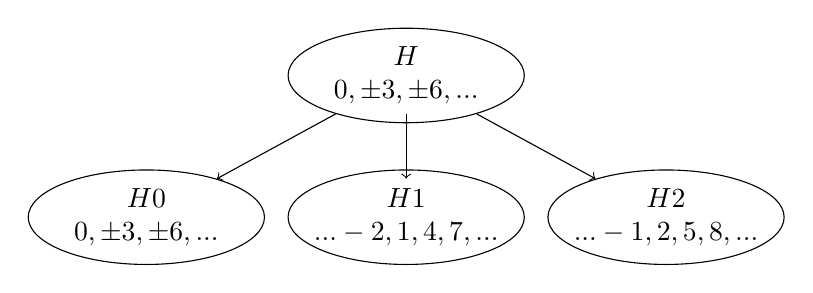
\begin{tikzpicture}[scale=0.6]
\draw (0, 3) circle[x radius=2.5cm, y radius=1cm] node[align=center] (H) {$H$ \\ $0, \pm 3, \pm 6, ...$}
      (-5.5, 0) circle[x radius=2.5cm, y radius=1cm] node[align=center] (H0) {$H0$ \\ $0, \pm 3, \pm 6, ...$}
      (0, 0) circle[x radius=2.5cm, y radius=1cm] node[align=center] (H1) {$H1$ \\ $... -2, 1, 4, 7, ...$}
      (5.5, 0) circle[x radius=2.5cm, y radius=1cm] node[align=center] (H2) {$H2$ \\ $... -1, 2, 5, 8, ...$};
\draw[->] (H) edge (H0)
          (H) edge (H1)
          (H) edge (H2);
\end{tikzpicture}
\caption{Right coset. For the additive group of integers, the subgroup $H$ contains all multiples of 3. Use 0, 1, 2 to add all these multiples, we get three non-overlapping sets. It is exactly one partition of integers.}
\label{fig:right-cosets-Z3}
\end{figure}

As shown in figure \ref{fig:right-cosets-Z3}, $Z$ is the additive group of integers. Set $H$ contains all multiples of 3, $0, \pm 3, \pm 6, ...$. It forms a subgroup under the addition. We use 0 in $Z$ to add from right\footnote{As the additive group of integers is Abelian, the addition is commutative, therefore, the left and right cosets are same.} to every element in $H$, which gives $H0$. Obviously, the result equals to $H$. It contains all the remainders of 0 modulo 3, denoted as [0]. Adding 1 in $Z$ from right to every element in $H$ gives $H1$. It contains all remainders of 1 modulo 3, denoted as [1]; Adding 2 in $Z$ from right to every element in $H$ gives $H1$. It contains all remainders of 2 modulo 3, denoted as [2]. If adding 3 to every elements in $H$, the result is as same as $H0$. In fact, whatever element $a$ we choose from $H0$ to generate a right coset $Ha$, it is always as same as $H0$; whatever element $b$ we choose from $H1$ to generate a right coset $Hb$, it is always as same as $H1$; whatever element $c$ we choose from $H2$ to generate a right coset $Hc$, it is always as same as $H2$. Put the three right cosets $H0$, $H1$, and $H2$ together, the result is exactly all the integers $Z$. It is a partition of $Z$: [0], [1], [3].

\begin{figure}[htbp]
\centering
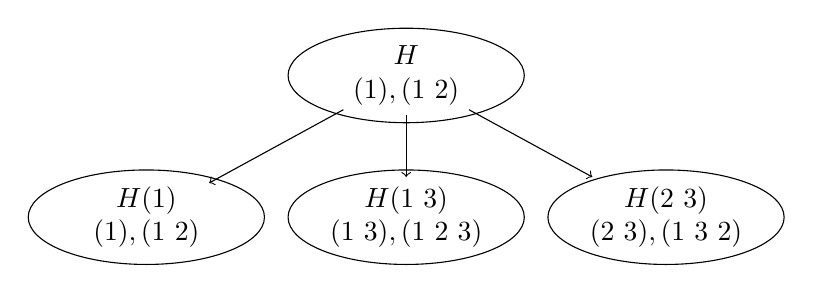
\begin{tikzpicture}[scale=0.6]
\draw (0, 3) circle[x radius=2.5cm, y radius=1cm] node[align=center] (H) {$H$ \\ $(1), (1\ 2)$}
      (-5.5, 0) circle[x radius=2.5cm, y radius=1cm] node[align=center] (H1) {$H(1)$ \\ $(1), (1\ 2)$}
      (0, 0) circle[x radius=2.5cm, y radius=1cm] node[align=center] (H13) {$H(1\ 3)$ \\ $(1\ 3), (1\ 2\ 3)$}
      (5.5, 0) circle[x radius=2.5cm, y radius=1cm] node[align=center] (H23) {$H(2\ 3)$ \\ $(2\ 3), (1\ 3\ 2)$};
\draw[->] (H) edge (H1)
          (H) edge (H13)
          (H) edge (H23);
\end{tikzpicture}
\caption{right cosets of a finite non-Abelian group.}
\label{fig:right-cosets-S3}
\end{figure}

Let's see another example about finite non-Abelian group. Consider a permutation group with degree 3.

$G = S_3 = \{(1), (1\ 2), (1\ 3), (2\ 3), (1\ 2\ 3), (1\ 3\ 2)\}$,

It has a subgroup $H = \{(1), (1\ 2)\}$. We use the identity permutation $(1)$ and another two permutations $(1\ 3)$, $(2\ 3)$ to multiply $H$ from right. It gives 3 right cosets:

\[
\begin{array}{rcl}
H(1) & = & \{(1), (1\ 2)\} \\
H(1\ 3) & = & \{(1\ 3), (1\ 2\ 3)\} \\
H(2\ 3) & = & \{(2\ 3), (1\ 3\ 2)\}
\end{array}
\]

We can use another three different elements to form the right cosets:

$H(1\ 2)$、$H(1\ 2\ 3)$、$H(1\ 3\ 2)$

Because $(1\ 2) \in H(1)$, $(1\ 2\ 3) \in H(1\ 3)$, $(1\ 3\ 2) \in H(2\ 3)$, therefore we have:

\[
\begin{array}{l}
H(1) = H(1\ 2) \\
H(1\ 3) = H(1\ 2\ 3) \\
H(2\ 3) = H(1\ 3\ 2)
\end{array}
\]

The subgroup $H$ partition the group $G = S_3$ into three disjoint right cosets $H(1)$、$H(1\ 3)$、$H(2\ 3)$. Putting these three right cosets together gets exactly $G$. They forms a partition of $G$.

\index{left coset}
Symmetric to right coset, we can also define left coset. Define the symmetric equivalence relation $\sim'$ as:

\[
a \sim' b \text{if and only if}\ b^{-1}a \in H
\]

The subset determined by equivalence relation $\sim'$ is called left coset of subgroup $H$. The left coset respect to element $a$ is denoted as $aH$. It contains all the elements in form of $ah, h \in H$ in $G$. As the multiplication operation for group may not be necessarily commutative, $\sim$ is not identical to $\sim'$ typically, therefore the left and right cosets are not same as well. However, there is a common property for both left and right cosets:

\begin{theorem}
For a given subgroup $H$, there are same numbers of left and right cosets. They are either infinity many, or the same finite numbers.
\end{theorem}

To prove this theorem, we can construct a map from the left coset to the right coset of $H$: $f: Ha \to a^{-1}H$. It's easy to verify this map is bijective (one to one correspondence). For all $Ha = Hb$, we have $ab^{-1} \in H$, and $(ab^{-1})^{-1} = ba^{-1} \in H$. Therefore, $a^{-1}H= b^{-1}H$. Since there exists one to one mapping, the numbers of left and cosets are same.

\index{index of subgroup}
With this theorem, we can use the number of the cosets (left or right) for a subgroup $H$ to define the \textbf{index} of $H$ in $G$.

In common cases, the right coset $Ha$ does not equal to the left coset $aH$. If they are same, such subgroup is called normal subgroup. It was Galois, who first introduced normal subgroups to analyze if equations are solvable in radicals.

\index{normal subgroup} \index{invariant subgroup}
\begin{definition}
For a group $G$, the subgroup $N$ is called \textbf{normal subgroup} (or invariant subgroup) if for every element $a$ in $G$, the equation:

\[
Na = aN
\]

holds. The left (or right) coset for a normal group is called \textbf{coset} of $N$.
\label{normal-subgroup}
\end{definition}

For the symmetric reason, a normal subgroup is also called the center of a group. We have two theorems to determine if a group is normal subgroup:

\begin{theorem}
For a group $G$, the subgroup $N$ is a normal subgroup (or invariant subgroup) if and only if for every element $a$ in $G$, equation:

\[
aNa^{-1} = N
\]

holds.
\end{theorem}

\begin{theorem}
For a group $G$, the subgroup $N$ is a normal subgroup (or invariant subgroup) if and only if for every element $a$ in $G$, $n$ in $N$, equation:

\[
ana^{-1} \in N
\]

holds.
\end{theorem}

For a normal subgroup $N$, all the cosets $\{aN, bN, cN, ...\}$ form a set. We define the multiplication for this set as:

\[
(xN)(yN) = (xy)N
\]

\index{quotient group}
It easy to verify that, the set of cosets form a group under this multiplication operation. This group is called \textbf{quotient group}, denoted as $G/N$. There is important relations between the normal subgroup, quotient group, and homomorphism. First, there is a homomorphism between $G$ and every its quotient group $G/N$. To proof it, we can construct a map $a \to aN, a \in G$. It is obvious that this map is surjective. For all elements $a, b$ in $G$, we have $ab \to abN = (aN)(bN)$. Therefore, it is a surjective homomorphism. This fact tell us, we can either use the subgroup, or quotient group to understand the property of $G$. To do that, let us define the concept of `kernel'.

\index{kernel}
\begin{definition}
If $f$ is a surjective homomorphism from group $G$ to another group $G'$, consider the identity element $e'$ in $G'$, its preimage under $f$ is a subset of $G$. This subset is called the \textbf{kernel} of the homomorphism.
\end{definition}

We have the following theorem. If $G$ is homomorphic to $G'$, then the kernal $N$ of the homomorphism is the normal subgroup of $G$. And the quotient group $G/N \cong G'$. A group is homomorphic to every of its quotient group, and from the abstract point of view, $G$ can only be homomorphic to its quotient groups. Sometimes, we find $G$ is homomorphic to $G'$, and we don't know well about the properties of $G'$. However, we are sure to be able to find a normal subgroup $N$ of $G$, that the properties of $G'$ are essentially identical to the quotient group $G/N$. We can see the importance of the normal subgroup and the quotient group. Galois did use this idea to figure out the way to define the equation group is solvable or not.

\begin{Exercise}
\Question{Proof theorem \ref{theorem:subgroup}, which determines if a subset forms a subgroup.}
\Question{List the left cosets for $H$ in figure \ref{fig:right-cosets-S3}.}
\end{Exercise}

\subsection{Lagrange's theorem}
\index{Lagrange}

Lagrange's theorem greatly demonstrated the power of abstract algebra. We can reveal the inner pattern of the abstract structure even knowing any concrete meanings of the group elements or their operations.

%\begin{figure}[htbp]
\begin{wrapfigure}{R}{0.4\textwidth}
 %\raggedright
 \centering
 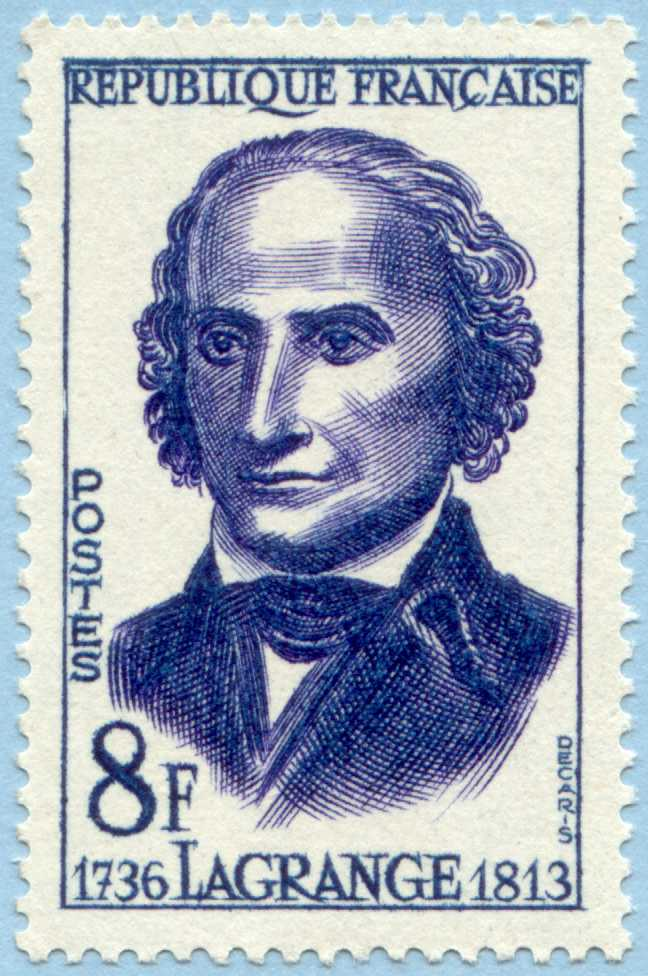
\includegraphics[scale=1.5]{img/lagrange.eps}
 \captionsetup{labelformat=empty}
 \caption{Stamp of Joseph-Louise Lagrange}
 \label{fig:Lagrange}
\end{wrapfigure}
%\end{figure}

Joseph-Louise Lagrange, was an mathematics, physics, and astronomer. He was born on January 25, 1736 in Turin, Italy. Lagrange was of Italian and French descent. His paternal great-grandfather was a French army officer who had moved to Turin, and married an Italian. His father, who had charge of the king's military chest and was Treasurer of the Office of Public Works and Fortifications in Turin. But before Lagrange grew up he had lost most of his property in speculations. A career as a lawyer was planned out for Lagrange by his father, and certainly Lagrange seems to have accepted this willingly. He later claimed: ``If I had been rich, I probably would not have devoted myself to mathematics.'' Lagrange studied at the University of Turin. At first he had no great enthusiasm for mathematics, finding Greek geometry rather dull.

It was not until he was seventeen that he showed any taste for mathematics – his interest in mathematics being first excited by a paper by Edmond Halley which he came across by accident. That paper introduced about the new calculus invented by Newton. Alone and unaided he threw himself into mathematical studies.

Starting in 1754, he worked on the problem of tautochrone, discovering a method of maximising and minimising functionals in a way similar to finding extrema of functions. Lagrange wrote several letters to Leonhard Euler between 1754 and 1756 describing his results. His work made him one of the founders of the calculus of variations. Euler was very impressed with Lagrange's results. As an accomplished mathematician, Lagrange was appointed to be an mathematics assistant professor at the Royal Military Academy of the Theory and Practice of Artillery in 1755. Already in 1756, Euler and Maupertuis, seeing Lagrange's mathematical talent, tried to persuade him to come to Berlin, but Lagrange had no such intention and shyly refused the offer.

In 1766, king Frederick of Prussia wrote to Lagrange expressing the wish of ``the greatest king in Europe'' to have ``the greatest mathematician in Europe'' resident at his court. Lagrange was finally persuaded and he spent the next twenty years in Prussia, where he produced not only the long series of papers published in the Berlin and Turin transactions, but also his monumental work, the {\em Mécanique analytique}.

Lagrange was a favourite of the king, who used frequently to discourse to him on the advantages of perfect regularity of life. The lesson went home, and thenceforth Lagrange studied his mind and body as though they were machines, and found by experiment the exact amount of work which he was able to do without breaking down. Every night he set himself a definite task for the next day, and on completing any branch of a subject he wrote a short analysis to see what points in the demonstrations or in the subject-matter were capable of improvement. He always thought out the subject of his papers before he began to compose them, and usually wrote them straight off without a single erasure or correction.

Nonetheless, during his years in Berlin, Lagrange's health was rather poor on many occasions, and that of his wife Vittoria was even worse. She died in 1783 after years of illness and Lagrange was very depressed.

In 1786, following Frederick's death, Lagrange accepted the offer of Louis XVI to move to Paris. In France he was received with every mark of distinction and special apartments in the Louvre were prepared for his reception, and he became a member of the French Academy of Sciences. It was about the same time, 1792, that the unaccountable sadness of his life and his timidity moved the compassion of 24-year-old Renée-Françoise-Adélaïde Le Monnier, daughter of his friend, the astronomer Pierre Charles Le Monnier. She insisted on marrying him, and proved a devoted wife to whom he became warmly attached.

In September 1793, the French revolution broke out. Under intervention of Antoine Lavoisier (known as the father of modern chemistry, who recognized and named oxygen and hydrogen), who himself was by then already thrown out of the Academy along with many other scholars, Lagrange was specifically exempted by name in the decree of October 1793 that ordered all foreigners to leave France. On May 4, 1794, Lavoisier, who had saved Lagrange from arrest, and 27 other tax farmers were arrested and sentenced to death and guillotined on the afternoon after the trial. According to a story, the appeal to spare Lavoisier's life so that he could continue his experiments was cut short by the judge, J. B. Coffinhal: ``The Republic has no need of scientists or chemists; the course of justice cannot be delayed.''. Lagrange said on the death of Lavoisier on May 8: ``It took only a moment to cause this head to fall and a hundred years will not suffice to produce its like.''\cite{Wiki-Lagrange}

After Coup of 18 Brumaire in 1799, Napoleon attained the power of France. He warmly encouraged science and mathematics studies in France, and was a liberal benefactor of them. He loaded Lagrange with honors and distinctions, appointed Lagrange as senator. In 1808, Napoleon made Lagrange a Grand Officer of the Legion of Honour and a Count of the Empire. Then honoured him with the Grand Croix of the Ordre of the Reunion on April 3, 1813. A week after, Lagrange died on April 10, 1813 at the age of 77. The funeral operation was pronounced by Laplace, represented the House of Lords, and Dean Lacépède represented the French Academy. The commemorative events were held in Italian universities.

Lagrange was the great mathematics and scientist in 18 to 19 Century. He made significant contributions to the fields of analysis, number theory, and both classical and celestial mechanics. Napoleon said ``Lagrange is the lofty pyramid of the mathematical science''. But above all his contribution, he is best known for his work on mechanics, where he transformed Newtonian mechanics into a branch of analysis, Lagrangian mechanics as it is now called, and presented the so-called mechanical "principles" as simple results of the variational calculus.

Lagrange made important progress in solving algebraic equations of any degree in the first decades in Berlin. He introduced a concept called Lagrange resolvents. The significance of this method is that it exhibits the already known formulas for solving equations of second, third, and fourth degrees as manifestations of a single principle. He failed to give a general formula for solutions of an equation of degree five and higher, because the auxiliary equation involved had higher degree than the original one. Nevertheless, Lagrange's idea already implies the concept of permutation group. The permutations made the resolvent invariant form a subgroup, and the order of the subgroup is the factor of the original permutation group. This is exactly the famous Lagrange's theorem in group theory. Lagrange is a pioneer of group theory. His thoughts were adopted and developed later by Abel and Galois, and was foundational in Galois theory.

Let us first introduce a lemma before Lagrange's theorem.

\begin{lemma}
For a subgroup $H$, there exists one to one mapping between $H$ and every right coset $Ha$.
\end{lemma}

As left and right cosets are symmetric, this lemma holds for left cosets as well. To prove it, we can build a map $f: h \to ha$. It is one to one mapping from the subgroup to right cosets because:

\begin{enumerate}
\item For every element $h$ in $H$, there exists unique image $ha$;
\item For every element $ha$ in $Ha$, it is the image of $h$ in subgroup $H$;
\item For any $h_1a = h_2a$, the equation $h_1 = h_2$ holds.
\end{enumerate}

From the existence of this one to one mapping, we know that for finite group $G$, the number of elements for any coset must equal to the order of the subgroup $H$. And according to the partition nature, every element in the group must be in some coset. Therefore, we have the insight between the subgroup $H$ and the finite group $G$ through cosets:

\index{Lagrange's theorem}
\begin{theorem}
\textbf{Lagrange's theorem}: For any finite group $G$, the order (number of elements) of every subgroup $H$ of $G$ divides the order of $G$.
\end{theorem}

\begin{proof}
First, we know that $G$ can be fully partitioned by the cosets of $H$; From the equivalence relation defined for coset, we know there is no overlap among them. If element $c$ belongs to both $Ha$ and $Hb$, then $c \sim a$, and $c \sim b$, therefore, $a \sim b$. Equation $Ha = Hb$ holds. And with the one to one mapping between the subgroup $H$ and cosets, we know the order of every coset equals to the order of $H$, which is $|H| = n$. Given the number of cosets is $m$ (which equals to the index of $H$), we finally get the result:

\[
|G| = mn
\]
\end{proof}

Note that there is a conversed question to Lagrange's theorem, whether every divisor of the order of a group is the order of some subgroup? This does not hold in general. Later we'll see such negative example in figure \ref{fig:group-graph} (c). The order of alternative group $A_4$ is 12, but it has no subgroup of order 6. We can deduce many interesting results from Lagrange's theorem.

\begin{corollary}
If $G$ is a finite group, the order of every element $a$ is a divisor of the order of $G$.
\end{corollary}

This is because $a$ generates a subgroup of order $n$, therefore $n$ divides $|G|$.

\begin{corollary}
If $G$ has prime order, then $G$ is cyclic.
\end{corollary}

This is because for every element $a$ excludes the identity element, the subgroup generated by $a$ has the same order as $G$. Therefore, $a$ is the generator of $G$, i.e. $G = (a)$.

\begin{corollary}
For every element $a$ in a finite group $G$, equation $a^{|G|} = e$ holds.
\label{corollary:Lagrange-elem-order}
\end{corollary}

This is because the order $n$ of $a$ divides $G$, let $|G| = nk$, we have:

\[
a^{|G|} = a^{nk} = (a^n)^k = e^k = e
\]

Lagrange's theorem in group theory can be used to prove the Fermat's little theorem in number theory. The theorem is named after Pierre de Fermat, who found in 1636. In a letter he wrote to a friend\footnote{Friend and confidant, French mathematician Frénicle de Bessy.} in October 18, 1640, Fermat first stated this theorem. It is called the ``little theorem'' to distinguish it from Fermat's last theorem. Euler provided the first published proof in 1736. But Leibniz had given virtually the same proof in an unpublished manuscript from sometime before 1683.

\index{Fermat's little theorem}
\begin{theorem}
\textbf{Fermat's little theorem}: If $p$ is prime, for any integer $a$ that $0 < a < p$, then $p$ can divides $a^{p-1}-1$.
\end{theorem}

\begin{proof}
Consider the multiplicative integer group modulo $p$. The group elements are all none zero residues modulo $p$. As $p$ is prime, therefore the group elements are 1, 2, ..., $p-1$. The identity element $e = 1$. The order of the group is thus $p-1$. According to the corollary \ref{corollary:Lagrange-elem-order} of Lagrange's theorem, we have:

\[
a^{p-1} = e
\]

Since the identity element is 1, this equation can be written as:

\[
a^{p-1} \equiv 1 \mod p
\]

Therefore, $p$ divides $a^{p-1} - 1$.
\end{proof}

Compare to this proof, the way to prove Fermat's little theorem in elementary theory of number is much complex (for example, section 5.2 - 5.4 in \cite{StepanovRose15}). Here we give another interesting combinatorial method called proof by counting necklace\cite{Wiki-FLT-proof}.

\begin{proof}
Consider there are pearls in $a$ different colors. we are going to make strings of length $p$, where $p$ is prime. Obviously there are total $a^p$ different strings, as every pearl can be chosen among $a$ colors, as we need make $p$ times selection.

For example there are pearls in two different colors $A$ red, and $B$ green. When make strings contain 5 pearls, that is $a = 2, p = 5$, there are total $2^5 = 32$ different strings:

\begin{verbatim}
  AAAAA, AAAAB, AAABA, ..., BBBBA, BBBBB.
\end{verbatim}

Corresponding to

\begin{verbatim}
  red-red-red-red-red,
  red-red-red-red-green,
  red-red-red-green-red,
  ...,
  green-green-green-green-red,
  green-green-green-green-green.
\end{verbatim}

We are going to prove that, among these $a^p$ strings, if remove $a$ strings that are all in the same color (in the above example, they are strings of \texttt{AAAAA} and \texttt{BBBBB}), the rest $a^p - a$ strings can be divided in several groups. Each group has exactly $p$ strings, thus $p$ divides $a^p - a$.

If we link the head and tail for every pearl string to make a necklace, some different strings will become same necklace. When a string can transform to the other by rotation, the two strings must form the same necklace. The following 5 strings form the same necklace for example:

\begin{verbatim}
  AAAAB, AAABA, AABAA, ABAAA, BAAAA.
\end{verbatim}

\begin{figure}[htbp]
  \centering
  \subcaptionbox{A necklace in 3 colors represents 7 different strings: \texttt{ABCBAAC}, \texttt{BCBAACA}, \texttt{CBAACAB}, \texttt{BAACABC}, \texttt{AACABCB}, \texttt{ACABCBA}, \texttt{CABCBAA}}[0.45\linewidth]{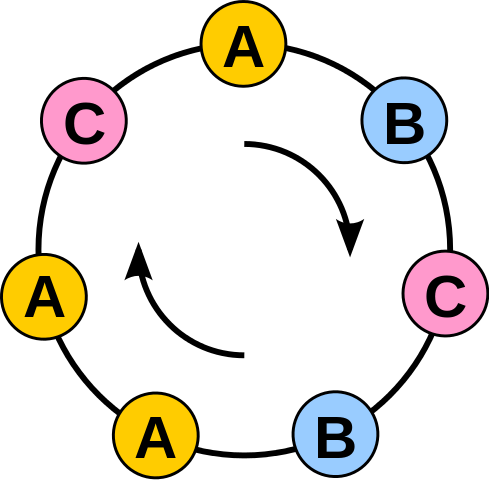
\includegraphics[scale=0.2]{img/bracelet-rotate.eps}} \quad
  \subcaptionbox{The necklace in same color only represent one string: \texttt{AAAAAAA}}[0.45\linewidth]{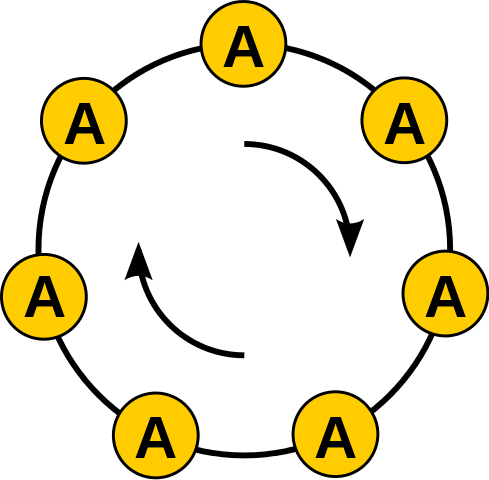
\includegraphics[scale=0.2]{img/bracelet-identical.eps}}
  \caption{Partition strings through necklace}
  \label{fig:bracelet}
\end{figure}

By this means, the 32 pearl strings in above example, can be partitioned into 5 necklaces in different colors and 2 necklaces in the same color:

\begin{verbatim}
  [AAABB, AABBA, ABBAA, BBAAA, BAAAB];
  [AABAB, ABABA, BABAA, ABAAB, BAABA];
  [AABBB, ABBBA, BBBAA, BBAAB, BAABB];
  [ABABB, BABBA, ABBAB, BBABA, BABAB];
  [ABBBB, BBBBA, BBBAB, BBABB, BABBB];
  [AAAAA];
  [BBBBB].
\end{verbatim}

How many strings can a necklace can represent? If a string $S$ can be split into several same sub-string $T$, while $T$ can't be split into the same sub-string any more, then the necklace $S$ represents $|T|$ different strings, where $|T|$ is the length of sub-string $T$. For example, string $S=$\texttt{ABBABBABBABB} can be split into sub-string $T=$\texttt{ABB}, while \texttt{ABB} can't be split any more. If we rotate a pearl per time, there are total 3 different results:

\begin{verbatim}
  ABBABBABBABB,
  BBABBABBABBA,
  BABBABBABBAB.
\end{verbatim}

There are not any other different strings besides these 3. Since the length of \texttt{ABB} is 3, further rotate must give the same result. Basically, there are two types for all the $a^p$ pearl strings. One type contains $a$ strings in same color; the rest are strings in different colors. However, as the length of the string $p$ is prime, it cannot be generated by duplicating sub-strings. Therefore, every necklace in different colors, represents $p$ different strings. There are total $a^p -a$ strings in different colors. They can be partitioned into groups by the necklaces being made. Each group contains exactly $p$ strings all can be represented with a same necklace. It tells us $p$ must divide $a^p-a = a^{p-1}$.

\end{proof}

The proof by counting necklaces might be the most straightforward method people developed. It need little mathematical knowledge. The key idea is two different counting methods must give the same result.

%\begin{figure}[htbp]
\begin{wrapfigure}{L}{0.35\textwidth}
  \centering %\raggedleft
 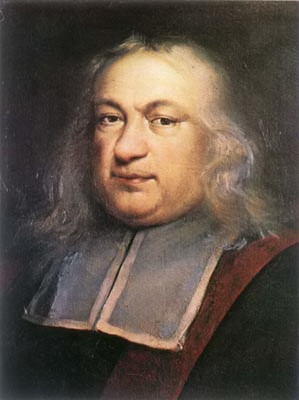
\includegraphics[scale=0.4]{img/Fermat.eps}
 \captionsetup{labelformat=empty}
 \caption{Pierre de Fermat, 1601-1665}
 \label{fig:Fermat}
\end{wrapfigure}
%\end{figure}

It took 100 years from the born of Fermat's little theorem to Euler's proof. It is not rare, but a typical Fermat style. Fermat's last theorem stimulated many talent mathematician. It took 358 years till the British mathematician Andrew Wiles solved it in 1995 successfully. The main tools Wiles used include elliptic curves, modularity theory, and Galois representations\cite{HanXueTao2009}. These conjectures left by Fermat are a rich mathematical treasure.

\vspace{5mm}

\index{Pierre de Fermat}

Pierre de Fermat was a French mathematician, born about August 1601. His father was a wealthy leather merchant. He became a lawyer at the Parlement of Toulouse French after grown up. In 1630, he bought the office of a councillor at the Parlement of Toulouse, one of the High Courts of Judicature in France, and was sworn in by the Grand Chambre in May 1631. He held this office for the rest of his life. Fermat thereby became entitled to change his name from Pierre Fermat to Pierre de Fermat. He was fluent in six languages. Fermat studied mathematics in his spare time. But the mathematical achievements made by Fermat were the peak of his time. Fermat's pioneering work in analytic geometry was circulated in manuscript form in 1636. It was based on results he achieved in 1629\footnote{The 8 pages paper, {\em Introduction to Plane and Solid Loci} was completed in 1630, but it was published posthumously in 1679, which was 14 years after Fermat's death.}. Together with René Descartes, Fermat was one of the two leading mathematicians of the first half of the 17th Century developed analytic geometry.

Fermat and Blaise Pascal laid the foundation for the theory of probability through their correspondence in 1654. From this brief but productive collaboration on the problem of points, they are now regarded as joint founders of probability theory. Fermat is credited with carrying out the first ever rigorous probability calculation.

In physics, Fermat refined the ancient Greek result about light and generalized to ``light travels between two given points along the path of shortest time'' now known as the principle of least time. For this, Fermat is recognized as a key figure in the historical development of the fundamental principle of least action in physics. The terms Fermat's principle and Fermat functional were named in recognition of this role. Fermat also contributed to the early development of calculus.

But Fermat's crowning achievement was in the theory of numbers. Fermat was inspired by the Diophantus's great work {\em Arithmetica} in ancient Greek. It was translated into Latin and published in France in 1621 by Claude Bachet. Fermat bought this book in Paris, and was deeply attracted by the puzzles in theory of numbers. One special point of this book was there were wide margin left in pages, it turned to be Fermat's `note book' when reading it. When studied the Diophantus' problem and answer, Fermat often got inspired to consider wider and deeper problems, then wrote his thoughts and comments in the margin.

Fermat published nearly nothing in his lifetime, although it is unbelievable from the view point of today. It was common in Fermat's time, that sometimes he wrote mails to his scholar friends about his findings. Some of the most striking of his results were found after his death on loose sheets of paper or written in the margins of works which he had read and annotated, and are unaccompanied by any proof. He was constitutionally modest and retiring, and does not seem to have intended his papers to be published. Fermat was totally driven by the strong curiousity to explore the mathematical mysteries. It's purely because of his treat mathematics study as a hobby. When he found the result that had never been touched, Fermat was truly exciting and self-satisfied. It was not significant to him to publish the result and get recognition\cite{HanXueTao2009}. Interestingly, this silent genius sometimes liked to tease people. He often challenged other mathematicians in mails by asking them to prove his discoveries.

\begin{wrapfigure}{R}{0.33\textwidth}
%\begin{figure}[htbp]
 \centering
 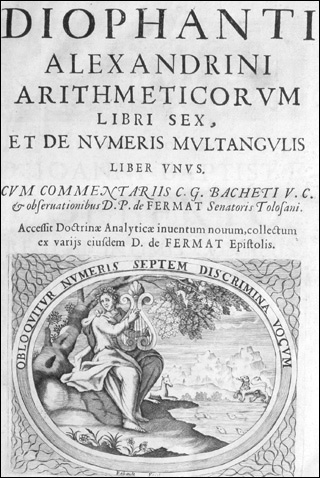
\includegraphics[scale=0.5]{img/Arithmetica.eps}
 \captionsetup{labelformat=empty}
 \caption{The 1670 edition of the Arithmetica of Diophantus, with Fermat's annotation.}
 \label{fig:Arithmetica}
%\end{figure}
\end{wrapfigure}

When Fermat died in Jan, 1665, his research results were scattered here and there. His son Clément-Samuel Fermat spent 5 years to collect Fermat's mails and notes, then produced a special edition of Arithmetica contained his father's achievement. On the cover page, it printed ``augmented with Fermat's commentary''. This edition includes 48 comments by Fermat. In 1679, Samuel collected and published the second volume of Fermat's work. His research results were finally circulated, which greatly enriched the mathematics in the 17th Century, and impact the development of mathematics later.

Before Fermat, the theory of numbers was basically a collection of problems. It was Fermat who first systematically studied the theory of numbers. He proposed a large number of theorems, and introduced generalized methods and principles, thus brought the theory of numbers to the modern development. It can be said that it is Fermat's systematic work that the theory of numbers really began to become a branch of mathematics. With his gift for number relations and his ability to find proofs for many of his theorems, Fermat essentially created the modern theory of numbers. He was called the "father of modern number theory." Before Gauss's {\em Arithmetic Research}, the development of number theory was originally driven by Fermat.

However, for many propositions conjectured, Fermat only provided some key part, or even without any proof. Some of them were found wrong\footnote{For example Fermat number, named after Fermat who first studied them in 1640, is a positive number of the form $2^{2^n}+1$. Fermat claimed all such numbers are primes. It is true when $n$ is 0, 1, 2, 3, 4. The corresponding numbers are 3, 5, 17, 257, 65537. However, in 1732 Euler calculated that $2^{2^5} + 1 = 641 \times 6700417$, is not a prime number. As of 2017, people have found 243 negative examples, without finding the 6th Fermat prime number. It is still a unsolved conjecture whether there are any other Fermat primes.}. Before given the strict mathematical proof, these propositions could only be called conjecture. Most of them were later solved by Euler. What's more, Euler greatly developed the theory of numbers on top of Fermat's work.

The Euler theorem in theory of numbers, is more generic than Fermat's little theorem. Euler did not satisfied after successfully proved Fermat's little theorem. What if $p$ is not prime? After carefully studied the general condition that covered composite numbers, Eular found and proved the following theorem.

\index{Euler Theorem} \index{Euler function}
\begin{theorem}
\textbf{Euler theorem}: If $0 < a < n$, $a$ and $n$ are coprime, then $n$ divides $a^{\upphi(n)} - 1$.
\end{theorem}

Where $\upphi(n)$ is Euler function\footnote{Also know as Euler totient function, or Euler $\upphi(n)$ function.}. It is defined as the number of all positive integers that less than $n$, and coprime to $n$.

\[
\upphi(n) = |\{i | 0 < i < n\ \text{and}\ gcd(i, n) = 1 \}|
\]

Euler proved this theorem with the method in elementary theory of numbers. There is a elegant proof by using Lagrange's theorem in group theory.

\begin{proof}
Consider the none zero residues modulo $n$. We pick out all the mutually inverse residues under the multiplication modulo $n$. They form a multiplicative group modulo $n$. From the definition of Euler $\upphi$ function, the value of $\upphi(n)$ is the number of all positive integers that less than $n$ and coprime to $n$. While these positive numbers are exactly the elements of the multiplicative group. Thus the order of this group is $\upphi(n)$. From the corollary \ref{corollary:Lagrange-elem-order} of Lagrange's theorem, we have:

\[
a^{\upphi(n)} = e
\]

Therefore, $a^{\upphi(n)} \equiv 1 \mod n$, which immediately gives the result, $n$ divides $a^{\upphi(n)} - 1$.
\end{proof}

Let us see an example. Below is the multiplication table for all the none zero residues modulo 10. We can located the identity element 1, and mark the cells underline. Then from that cell, along with the row and column, we can find two numbers, marked in bold. Their modulo product is 1, and both are coprime to 10. On the other hand, for every residue number that is not coprime to 10, the row and column where it is also contain 0. But 0 is not group element. We can see that all the residues that are coprime to 10 are exactly the group elements 1, 3, 7, 9.

\vspace{5mm}
\definecolor{Gray}{gray}{0.9}
\newcolumntype{g}{>{\columncolor{Gray}}c}
\begin{tabular}{c|g|c|g|c|c|c|g|c|g|}
  & \textbf{1} & 2 & \textbf{3} & 4 & 5 & 6 & \textbf{7} & 8 & \textbf{9} \\
\hline
\rowcolor{Gray}
\textbf{1} & \cellcolor{gray} \underline{1} & 2 & 3 & 4 & 5 & 6 & 7 & 8 & 8 \\
\hline
2 & 2 & 4 & 6 & 8 & 0 & 2 & 4 & 6 & 8 \\
\hline
\rowcolor{Gray}
\textbf{3} & 3 & 6 & 9 & 2 & 5 & 8 & \cellcolor{gray}\underline{1} & 4 & 7 \\
\hline
4 & 4 & 8 & 2 & 6 & 0 & 4 & 8 & 2 & 6 \\
\hline
5 & 5 & 0 & 5 & 0 & 5 & 0 & 5 & 0 & 5 \\
\hline
6 & 6 & 2 & 8 & 4 & 0 & 6 & 2 & 8 & 4 \\
\hline
\rowcolor{Gray}
\textbf{7} & 7 & 4 & \cellcolor{gray} \underline{1} & 8 & 5 & 2 & 9 & 6 & 3 \\
\hline
8 & 8 & 6 & 4 & 2 & 0 & 8 & 6 & 4 & 2 \\
\hline
\rowcolor{Gray}
\textbf{9} & 9 & 8 & 7 & 6 & 5 & 4 & 3 & 2 & \cellcolor{gray} \underline{1} \\
\hline
\end{tabular}
\vspace{5mm}

Given a integer $n$, how to evaluate Euler function? As any integer greater than 1 can be factored as power of prime numbers, let us first see how to evaluate $\upphi(p^m)$ for the $m$ power of a prime $p$. We are going to count how many numbers from 1 to $p^m - 1$ are coprime to $p^m$. We can easily do this by removing the multiples of $p$. These numbers are $p, 2p, 3p, ..., p^m - p$. Divide them by $p$, gives the nature number sequence $1, 2, 3, ..., p^{m-1} - 1$. We immediately know there are $p^{m-1} - 1$ numbers. On top of this, we deduce the value of Euler function for the power of prime number as:

\[
\begin{array}{rcl}
\upphi(p^m) & = & (p^m - 1) - (p^{m-1} - 1) \\
            & = & p^m - p^{m-1} \\
            & = & p^m(1-\dfrac{1}{p})
\end{array}
\]

We next consider number in form of $n = p^uq^v$, which is product of power of different prime numbers. We need first remove all multiples of $p$, then remove all multiples of $q$. But there are numbers that are the multiples of both $p$ and $q$. They are removed twice. We need add these multiples of $pq$ back (Principle of inclusion and exclusion in combinatorics). Thus we have:

\[
\begin{array}{rcl}
\upphi(p^uq^v) & = & (n - 1) - (\dfrac{n}{p} - 1) - (\dfrac{n}{q} - 1) + (\dfrac{n}{pq} - 1) \\
          & = & n(1 - \dfrac{1}{p})(1 - \dfrac{1}{q}) \\
          & = & p^u(1 - \dfrac{1}{p})q^v(1 - \dfrac{1}{q}) \\
          & = & \upphi(p^u)\upphi(p^v)
\end{array}
\]

Particularly when both $u$ and $v$ are 1, we have $\upphi(pq) = \upphi(p)\upphi(q)$. We can expand this result to multiple powers of prime numbers. Given $n = p_1^{k_1}, p_2^{k_2}...p_m^{k_m}$, the Euler function can be evaluated as:

\[
\begin{array}{rcl}
\upphi(n) & = & n(1-\dfrac{1}{p_1})(1-\dfrac{1}{p_2})...(1-\dfrac{1}{p_m}) \\
    & = & \upphi(p_1^{k_1})\upphi(p_2^{k_2})...\upphi(p_m^{k_m})
\end{array}
\]

We can develop the fast evaluation algorithm from this result. We leave this as an exercise in this chapter.

\vspace{5mm}

\index{Euler}

Leonhard Euler was a great Swiss mathematician and scientist. He is held to be one of the greatest mathematician in the history together with Archimedes, Newton, and Gauss. Euler was born on April 15, 1707 in Basel Switzerland. As a paster, his father urged him to study theology and became paster too. Euler enrolled at the University of Basel at the age of 13 with major of philosophy and theology. During that time, he was receiving Saturday afternoon lessons from Johann Bernoulli, the foremost mathematician in Europe. Bernoulli quickly discovered Euler's incredible talent for mathematics, and convinced his father that Leonhard was destined to become a great mathematician.

%\begin{wrapfigure}{R}{0.4\textwidth}
\begin{figure}[htbp]
 \centering
 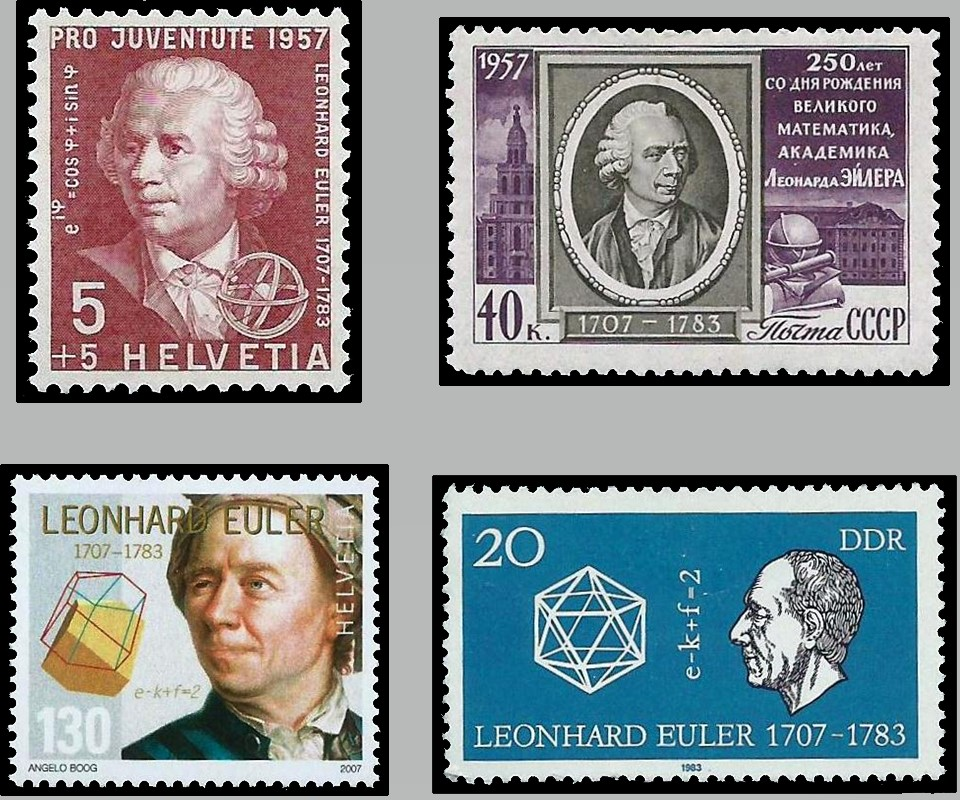
\includegraphics[scale=0.4]{img/euler.eps}
 \captionsetup{labelformat=empty}
 \caption{Stamps commemorating Leonhard Euler (1707 - 1783)}
 \label{fig:Leonhard-Euler}
\end{figure}
%\end{wrapfigure}

In 1727, Euler became a member of Imperial Russian Academy of Sciences in Saint Petersburg. He devoted himself to research work and later became the head of mathematics department after his friend, Daniel Bernoulli left for Basel. During the 14 years in Russia, Euler studied analytics, number theory, and mechanics. In 1747, Euler took up a position at the Berlin Academy, which he had been offered by Frederick the Great of Prussia. He lived for 25 years in Berlin, where he wrote over 380 articles. During this time, his research was more extensive, involving planetary motion, rigid body movement, thermodynamics, ballistics, and demography. These work were closely connected with his research in mathematics. Euler made groundbreakings in differential equations, and surface differential geometry. After the political situation in Russia stabilized after Catherine the Great's accession to the throne, in 1766 Euler accepted an invitation to return to the St. Petersburg Academy. He spent the rest of his life in Russia.

Euler worked in almost all areas of mathematics, such as geometry, infinitesimal calculus, trigonometry, algebra, and number theory, as well as continuum physics, lunar theory and other areas of physics. He is a seminal figure in the history of mathematics; From the age of 19 till he died at 76, he published huge number of research papers and books in half a Century. Euler's name is associated with almost every area in mathematics. He was the top productive mathematician in the history with a total of 856 papers, and 31 books. And these did not counted the loss of the fire in St. Petersburg in 1771. (Euler's record was broken by Hungarian mathematician Paul Erdős in the 20th Century, who published 1525 papers and 32 books) \cite{Wiki-Euler}.

Euler had unbelievable strong willpower. His right eye lost sight from a fever. Three years later, he become almost blind in his right eye. But even worse, his left eye lost sight too in 1771. But Euler rather blamed the painstaking work on cartography he performed for his condition. Just as deafness did not stop Beethoven’s music creation, blindness did not stop Euler’s mathematical exploration\cite{HanXueTao2009}. Euler remarked on his loss of vision, ``Now I will have fewer distractions.'' As he compensated for it with his mental calculation skills and exceptional memory. He could not only remember the first 100 prime numbers, but also their square, cubic, and even higher power. He can also perform complex mental arithmetic. With the aid of his scribes, Euler's productivity on many areas of study actually increased. He produced, on average, one mathematical paper every week in the year 1775. Half of Euler's work was dictated after his eyes were completely blind. The French physicist François Arago said ``Euler calculated without any apparent effort, just as men breathe, as eagles sustain themselves in the air.''. Euler could work in any bad environment. He often held the child on the lap to complete the papers, regardless of any noise around.

Among Euler's work, there are difficult monographs, and readings for the general public. Euler wrote over 200 letters to a German Princess in early 1760s, which were later compiled into a best-selling volume entitled Letters of Euler on different Subjects in Natural Philosophy Addressed to a German Princess. This book became more widely read than any of his mathematical works and was published across Europe and in the United States. The popularity of the "Letters" testifies to Euler's ability to communicate scientific matters effectively to a lay audience, a rare ability for a dedicated research scientist. Euler also wrote a course on elementary algebra for readers of non-mathematics background, which is still in print today. Many popular mathematical notations we are using today were carefully introduced by Euler, for example $\pi$ (1736), the imaginary unit$i$ (1777), the base of the natural logarithm $e$, now also known as Euler's number (1748), circular function $sin$, $cos$ (1748), and $tg$ (1753), $\Delta x$ (1755), summation $\sum$ (1755), function $f(x)$ (1734) and so on\cite{HanXueTao2009}.

On September 18, 1783, after a lunch with his family, Euler was discussing the newly discovered planet Uranus and its orbit with a fellow academician. As usual, he played with one of his granddaughter while having tea. Suddenly, the pipe drop from his hand. He said ``My pipe'', then bent over to pick it, but he was not able to stand, uttered only ``I am dying'' before he lost consciousness. ``He ceased to calculate and to live.''\footnote{In the eulogy for the French Academy, French mathematician and philosopher Marquis de Condorcet wrote this.}

\vspace{5mm}

\index{RSA cryptosystem}

Fermat little theorem is widely used in our everyday life, from internet shopping to electronic payment. In 1976, professor Whitfield Diffie and Martin Hellman in Stanford University developed the concept of asymmetric public-private key cryptosystem. In 1977, Ron Rivest, Adi Shamir, and Leonard Adleman in Massachusetts Institute of Technology (MIT) developed a one-way function that was hard to invert based on theory of numbers. The algorithm is now known as RSA – the initials of their surnames in same order as their paper.

The key asymmetry concept of RSA is based on the fact that we can easily create a composite numbers from two large prime numbers, while there is practical difficulty to factor them. This is known as the {\em factoring problem}. For a large number of over 200 digits, even the most powerful super computer will cost time longer than the age of universe. In order to construct a encrypt key hard to break, we need a method that can find the large prime numbers fast. However, people do not know the exact pattern about how prime numbers distributed in nature numbers. There is no formula to enumerate prime numbers. The brute force method is to randomly pick a number $n$, then examine from 1 to $\sqrt{n}$, check if all do not divide $n$. But this primality test method is very ineffective. The time will also exceed the age of universe. A better method is the Eratosthenes sieve algorithm. We first enumerate all numbers from 2 to $n$. Start from 2, removal all multiples of 2, then remove all multiples of 3... Repeat this every time from the next number that is not filtered out, till the number not greater than $\sqrt{n}$. This process gives all the prime numbers to $n$. However, it is still applicable for small $n$, but can't serve for the large number primality test.

Interestingly, Fermat's little theorem provides a way for fast primality test. For a large number $n$, we can randomly select a positive integer $a$ less than it as a `witness'. Then check if the remainder of $a^{n-1}$ modulo $n$ is 1. If not 1, $n$ must not be prime number according to Fermat's little theorem. Otherwise if it is 1, then $n$ may be a prime number.

The {\em Fermat primality test} algorithm (also known as Fermat test) based on this idea can be described as below:

\begin{algorithmic}
\Function{primality}{$n$}
  \State Random select a positive integer $a < n$
  \If{$a^{n-1} \equiv 1 \mod n$}
    \State \Return prime number
  \Else
    \State \Return composite number
  \EndIf
\EndFunction
\end{algorithmic}

We needn't compute the exact value of $n-1$ power of $a$, then divide $n$ to get the remainder. We can use modular arithmetic to speed up. The intermediate result can be largely re-used. After we calculate $b = a^2 \mod n$, we can next get $b^2 \mod n$, which equals to $a^4 \mod n$. For example, when evaluate $a^{11} \mod n$, since:

\[
a^{11} = a^{8 + 2 + 1} = ((a^2)^2)^2a^2a \mod n
\]

What have to calculated are only $a^2 \mod n$, $(a^2)^2 \mod n$, and $((a^2)^2)^2 \mod n$. Basically, we can express $n$ in binary format, and only iterate calculate the modular product for the digits of 1. This is a algorithm with complexity of $O(\lg n)$. Fermat test is very fast because of this.

However, even a number passed Fermat test, it is not necessarily prime number. For example 341 = 11 $\times$ 31 is a composite number, but $2^{340} \equiv 1 \mod 341$ can pass the Fermat test. To reduce the probability of such failure, people developed many improvements. The first improvement is to increase the number of witness. We can prove that, if a number does not pass Fermat test, then there exist at least half of $n$ numbers that can't pass too (\cite{Algorithms-DPV}, pp26).

\begin{theorem}
For positive integer $a$ less than $n$, and coprime with $n$, if $a^{n-1} \not\equiv 1 \mod n$, then for all selected $a < n$, it also holds for at least half.
\end{theorem}

\begin{figure}[htbp]
\centering
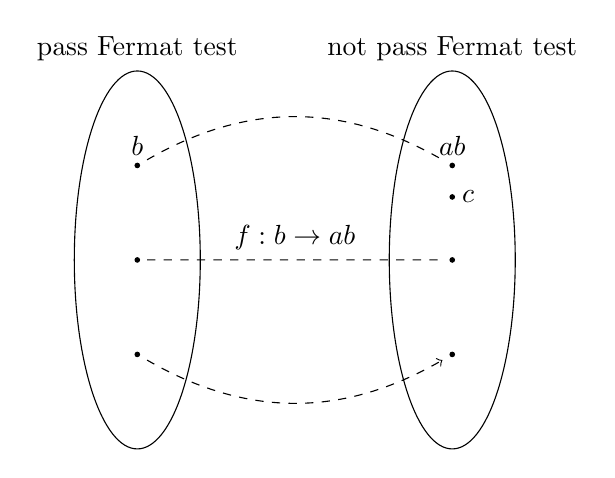
\begin{tikzpicture}[scale=0.8]
\draw (0, 0) circle[x radius=1cm, y radius=3cm]
      (5, 0) circle[x radius=1cm, y radius=3cm];
\path (0, 3) node[above] {pass Fermat test}
      (5, 3) node[above] {not pass Fermat test};
\path (0, 0) node (b) {}
      (5, 0) node (fb) {}
      (0, 1.5) node (a) {}
      (5, 1.5) node (fa) {}
      (0, -1.5) node (c) {}
      (5, -1.5) node (fc) {};
\filldraw (0, 0) circle (1pt) node[above] {}
      (5, 0) circle (1pt) node[above] {}
      (0, 1.5) circle (1pt) node[above] {$b$}
      (5, 1.5) circle (1pt) node[above] {$ab$}
      (5, 1) circle (1pt) node[right] {$c$}
      (0, -1.5) circle (1pt) node[above] {}
      (5, -1.5) circle (1pt) node[above] {};
\draw[dashed, ->] (b) to node [above] {$f: b \to ab$} (fb)
      (a) to [bend left] (fa)
      (c) to [bend right] (fc);
\end{tikzpicture} \\
Set $\{1, 2, ..., n-1\}$
\caption{Map from the set that pass Fermat test to the set that does not}
\label{fig:Fermat-test}
\end{figure}

\begin{proof}
If for some $a$ that $a^{n-1} \not\equiv 1 \mod n$ holds, then for any witness $b$ that passes Fermat test (It means $b^{n-1} \equiv 1 \mod n$), we can create a negative case for Fermat test $ab$.

\[
(ab)^{n-1} \equiv a^{n-1}b^{n-1} \equiv a^{n-1}1 \not\equiv 1 \mod n
\]

And because $i \neq j$, we have $a \cdot i \not\equiv a \cdot j$, therefore, all these negative cases are not same.

As shown in figure \ref{fig:Fermat-test}, if there exists a number that can't pass Fermat test, then the positive cases are as same amount as the negative cases.
\end{proof}

If we select $k$ different witness and perform Fermat test, we can reduce the probability of failure that $n$ is not prime number to $\dfrac{1}{2^k}$. However, there exist such composite number $n$, that for any $a$ less than $n$ and coprime to $n$, $a^{n-1} \equiv 1 \mod n$ holds. It means whatever $a$ we selected, such composite number can pass Fermat test. Carmichael found first such number in 1910, that 561 = 3 $\times$ 11 $\times$ 17. This kind of numbers is called Carmichael numbers or Fermat pseudoprime\footnote{The Czech mathematician Václav Šimerka found the first 7 Fermat pseudoprimes: 561 = 3 $\times$7 $\times$11, 1105 = 5 $\times$13 $\times$7, 1729 = 7 $\times$13 $\times$19, 2465 = 5 $\times$17 $\times$29, 2821 = 7 $\times$13 $\times$31, 6601 = 7 $\times$23 $\times$41, 8911 = 7 $\times$19 $\times$67. However, his work was not well known to the people}. Erdős conjectured there are infinite many Carmichael numbers. In 1994, people proved for sufficient large $n$, there are at least $n^{2/7}$ Carmichael numbers from 1 to $n$. Thus explains Erdős' conjecture\cite{Wiki-Carmichael-number}.

The primality test algorithm in RSA is Miller-Rabin algorithm. It is also a probabilistic algorithm\footnote{There is a deterministic version of Miller-Rabin algorithm, but the correctness is on top of the generalized Riemann hypothesis (GRH)\cite{Wiki-Miller-Rabin}.}. According to the above theorem, if select more than 100 witnesses, the probability of failure is expected less than $\frac{1}{2^{100}}$. Donald Knuth commented ``far less, for instance, than the probability that a random cosmic ray will sabotage the computer during the computation!''

%TODO: Add RSA implementation in Appendix.

\vspace{5mm}

We summarized the relations for group, semigroup, monoid we introduced so far as the following diagram.

\begin{figure}[htbp]
\centering
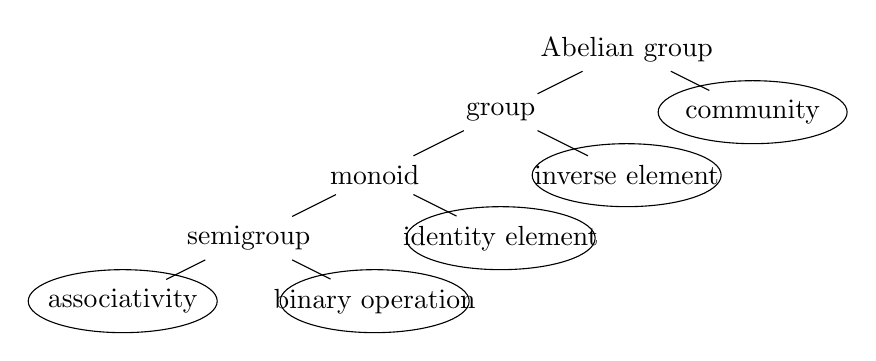
\begin{tikzpicture}[scale=0.8]
\draw (4, 2) node (abeliangroup) {Abelian group}
      (2, 1) node (group) {group}
      (0, 0) node (monoid) {monoid}
      (-2, -1) node (semigroup) {semigroup};
\draw (-4, -2) circle[x radius = 1.5cm, y radius = 0.5cm] node (assoc) {associativity}
      (0, -2) circle[x radius = 1.5cm, y radius = 0.5cm] node (binop) {binary operation}
      (2, -1) circle[x radius = 1.5cm, y radius = 0.5cm] node (unit) {identity element}
      (4, 0) circle[x radius = 1.5cm, y radius = 0.5cm] node (invert) {inverse element}
      (6, 1) circle[x radius = 1.5cm, y radius = 0.5cm] node (community) {community};
\draw (abeliangroup) to (community)
      (abeliangroup) to (group)
      (group) to (invert)
      (group) to (monoid)
      (monoid) to (unit)
      (monoid) to (semigroup)
      (semigroup) to (binop)
      (semigroup) to (assoc);
\end{tikzpicture}
\caption{group, semigroup, monoid}
\label{fig:groups}
\end{figure}

\begin{Exercise}
\Question{Today is Sunday, what day it will be after $2^{100}$ days?}
\Question{Given tow strings (character string or list), write a program to test if they form the same necklace.}
\Question{Write a program to realize Eratosthenes sieve algorithm.}
\Question{Extend the idea of Eratosthenes sieve algorithm, write a program to generate Euler $\upphi$ function values for all numbers from 2 to 100.}
\Question{Write a program to realize fast modular multiplication, and Fermat's primality test.}
\end{Exercise}

\section{Ring and Field}

\begin{wrapfigure}{R}{0.3\textwidth}
%\begin{figure}[htbp]
 \centering
 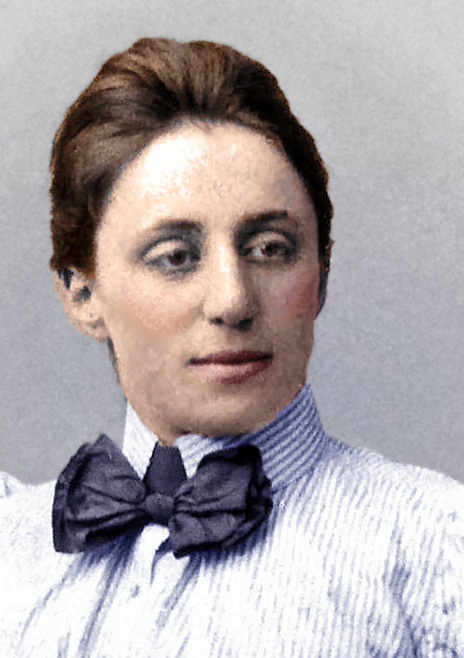
\includegraphics[scale=1]{img/Noether.eps}
 \captionsetup{labelformat=empty}
 \caption{Emmy Noether, 1882-1935}
 \label{fig:Noether}
%\end{figure}
\end{wrapfigure}

\index{Emmy Noether}

The modern theories of rings, fields, and abstract algebra was developed by German mathematician Emmy Noether. Noether was born to a Jewish family in Erlangen Germany on March 23, 1882. Her father was a mathematician in the University of Erlangen. She originally planned to teach French and English after passing the required examinations in 1900, but she chose instead to continue her studies at the University of Erlangen where her father lectured.

This was an unconventional decision. Two years earlier, the Academic Senate of the university had declared that allowing mixed-sex education would ``overthrow all academic order''. One of only two women in a university of 986 students, Noether was only allowed to audit classes rather than participate fully, and required the permission of individual professors whose lectures she wished to attend. Despite these obstacles, on 14 July 1903 she passed the graduation exam at a Realgymnasium in Nuremberg.

During the 1903–1904 winter semester, she studied at the University of Göttingen, attending lectures given by astronomer Karl Schwarzschild and mathematicians Hermann Minkowski, Otto Blumenthal, Felix Klein, and David Hilbert. Noether returned to Erlangen. She officially reentered the university in October 1904, and declared her intention to focus solely on mathematics. Under the supervision of Paul Gordan she wrote her dissertation. For the next seven years (1908–1915) she taught at the University of Erlangen's Mathematical Institute without pay only because she was a woman.

The mathematician Ernst Fischer was an important influence on Noether, in particular by introducing her to the work of David Hilbert. From 1913 to 1916 Noether published several papers extending and applying Hilbert's methods to mathematical objects such as fields of rational functions and the invariants of finite groups. This phase marks the beginning of her engagement with abstract algebra, the field of mathematics to which she would make groundbreaking contributions.

In the spring of 1915, Noether was invited to return to the University of Göttingen by David Hilbert and Felix Klein. Their effort to recruit her, however, was blocked by the philologists and historians among the philosophical faculty: Women, they insisted, should not become privatdozenten. Hilbert responded with indignation, stating, ``I do not see that the sex of the candidate is an argument against her admission as privatdozent. After all, we are a university, not a bath house.''

During her first years teaching at Göttingen she did not have an official position and was not paid; her family paid for her room and board and supported her academic work. Her lectures often were advertised under Hilbert's name, and Noether would provide ``assistance''.

Soon after arriving at Göttingen, however, she demonstrated her capabilities by proving the theorem now known as Noether's theorem, which shows that a conservation law is associated with any differentiable symmetry of a physical system. American physicists Leon M. Lederman and Christopher T. Hill argue in their book Symmetry and the Beautiful Universe that Noether's theorem is ``certainly one of the most important mathematical theorems ever proved in guiding the development of modern physics, possibly on a par with the Pythagorean theorem''.

In 1919 the University of Göttingen allowed Noether to proceed with her habilitation. Noether was not paid for her lectures until she was appointed to the special position in 1923.

Noether's work in algebra began in 1920. She published the important paper {\em Theory of Ideals in Ring Domains} in 1921. This revolutionary work gave rise to the term ``Noetherian ring'' and the naming of several other mathematical objects as Noetherian. In 1931, Noether's student, Dutch mathematician Van der Waerden published {\em Moderne Algebra}, a central text in the field developed by Noether. Although Noether did not seek recognition, Van der Waerden included a note ``based in part on lectures by E. Artin and E. Noether''. This classic book influenced a generation of young mathematicians in that time. In Göttingen, Noether supervised more than a dozen doctoral students. In November 1932, Noether delivered one hour speech at the 9th International Congress of Mathematicians in Zürich. with 800 attendees. Apparently, this prominent speaking position was a recognition of the importance of her contributions to mathematics. The 1932 congress is sometimes described as the high point of her career.

However, the huge reputation and recognition did not improve her difficult situation as a woman. Her colleagues were frustrated for the fact that she was not elected to the Göttingen academy of sciences and was never promoted to the position of full professor. Her frugal lifestyle was due to being denied pay for her work; However, even after the university began paying her a small salary in 1923, she continued to live a simple and modest life.

After Hitler gain the power of German, Nazi administration persecuted Jews intensified. In 1929, Noether was taken out of the apartment where she lived. In April 1933, Noether was forced to stop teaching at the University of Göttingen. Several of Noether's colleagues, including Max Born and Richard Courant, also had their positions revoked. Noether accepted the decision calmly, providing support for others during this difficult time. Hermann Weyl later wrote that ``Emmy Noether—her courage, her frankness, her unconcern about her own fate, her conciliatory spirit—was in the midst of all the hatred and meanness, despair and sorrow surrounding us, a moral solace.''

As dozens of newly unemployed professors began searching for positions outside of Germany. Albert Einstein and Hermann Weyl were appointed by the Institute for Advanced Study in Princeton, while others worked to find a sponsor required for legal immigration. Although Noether was the world famous mathematician, it was very hard for her to get a position from large institutions as a women. After a series of negotiations with the Rockefeller Foundation, a grant to Bryn Mawr College in the United States was approved for Noether and she took a position there, starting in late 1933. This is a girl's University, and Noether lectured there as a visiting scholar. Although she was invited to Princeton University to give lectures, she remarked that she was not welcome at ``the men's university, where nothing female is admitted''.

In April 1935, doctors discovered a tumor in Noether's pelvis. She was died after the surgery on April 14 at the age of 53.

Noether is best remembered for her contributions to abstract algebra. Nathan Jacobson wrote that: ``The development of abstract algebra, which is one of the most distinctive innovations of twentieth century mathematics, is largely due to her.''. She sometimes allowed her colleagues and students to receive credit for her ideas, helping them develop their careers at the expense of her own. She was described by Pavel Alexandrov, Albert Einstein, Jean Dieudonné, Hermann Weyl and Norbert Wiener as the most important woman in the history of mathematics\cite{Wiki-Noether}.

\subsection{Ring}
\index{ring}
Let us see how ring is defined in mathematics.

\begin{definition}
A ring is a set $R$ that satisfies below \textbf{ring axioms}:
\begin{enumerate}
\item $R$ is a additive group, it means $R$ forms an abelian group under the addition operation defined on it;
\item There is multiplication defined for $R$, and $R$ is close under this multiplication operation;
\item The multiplication is associative. For all $a, b, c$, equation $(ab)c = a(bc)$ holds;
\item Multiplication is distributive with respect to addition, meaning that, for all $a, b, c$, we have:
\[
\begin{array}{l}
a(b + c) = ab + ac \\
(b + c)a = ba + ca
\end{array}
\]
\end{enumerate}
\end{definition}

\index{commutative ring}
Obviously, all integers form a ring under the addition and multiplication. Other examples are polynomials and matrix form ring under the addition and multiplication. The ring definition only requires the addition operation is commutative, thus the ring is an abelian group under addition. It does not have such requirement for multiplication. When the ring multiplication is also commutative, we call it \textbf{commutative ring}. In commutative ring, for positive integer $n$ and any two elements, the following equation holds:

\[
a^nb^n = (ab)^n
\]

The ring definition does not require a identity element for the multiplication too. If there exists an element $e$ in $R$, it satisfies the below equations for all elements:

\[
ea = ae = a
\]

We call $e$ the \textbf{unity} (multiplicative identity element) of the ring. A ring may not necessarily have unity. Traditionally, we use 1 to represent the unity. It is just a symbol, but not means the actual number 1. With unity, we can also define inverse element. If $ab = ba = 1$, we say $b$ is the inverse element of $a$. According to the group property, we know that if the ring has an identity element for multiplication, it is unique. If an element is invertible, the inverse element is also unique. While not all elements are invertible, for example, the integer ring has unity, but except for $\pm 1$, all other integers are not invertible. We call the invertible element a \textbf{unit}.

From the distributive axiom, we have:

\[
(a - a)a = aa - aa = 0
\]

It means, if either $a$ or $b$ is 0, then $ab = 0$. But the inverse proposition does not hold. We can not deduce from $ab =0$ to either $a$ or $b$ is 0. Let's see a negative example. Consider the residue class modulo $n$, where the addition operation is modulo addition: $[a] + [b] = [a + b]$, which takes modulo $n$ on top of the sum. It forms an abelian addition group. The multiplication modulo $n$ is defined as: $[a][b] = [ab]$, which takes modulo $n$ on top of the product. It's easy to verify that this is a ring, named as residue ring modulo $n$.

If $n$ is not prime, for example 10, we can multiply two none zero elements $[5][2] = [5 \times 2] = [0]$. In fact, any two factors of $n$, their modulo product must be zero.

\index{zero divisor}
In a ring, if there exists $a \neq 0, b \neq 0$, but $ab = 0$, we call $a$ is a \textbf{left zero divisor}, and $b$ is a \textbf{right zero divisor} of the ring. For the commutative ring, a left zero divisor is also a right zero divisor. Of course, it's possible there is no zero divisor, for example the integer ring. For $ab = 0$, we can deduce either $a$ or $b$ is 0 only if there is no zero divisor in the ring. And we have the following theorem:

\begin{theorem}
For a ring without zero divisor, the following two cancellation rules hold.
\begin{itemize}
\item If $a \neq 0$, and $ab = ac$, then $b = c$;
\item If $a \neq 0$, and $ba = ca$, then $b = c$;
\end{itemize}
\end{theorem}

Conversely, if one cancellation rule hold in a ring, then the other cancellation rule also hold, and there is no zero divisor in this ring.

\index{integral domain}
So far, we introduced three additional conditions: (1) The multiplication is commutative; (2) There exists unity; (3) No zero divisor. A ring that satisfies these three additional constraints is called \textbf{integral domain} (nonzero commutative ring). It's obvious that integer ring is an integral domain.

\index{semiring}
The ring constraints are strong. Sometimes, we needn't the additive inverse. By weakening the limitation, we obtain the \textbf{semiring}.

\begin{definition}
A set $R$ under the addition and multiplication forms a semiring if it satisfies the following axioms:
\begin{enumerate}
\item $R$ forms a commutative monoid under addition, and there exists the identity element 0;
\item $R$ forms a monoid under multiplication, and there exists the identity element 1 (unity);
\item Multiplication is distributive with respect to addition. For any $a, b, c$:
\[
\begin{array}{l}
a(b + c) = ab + ac \\
(b + c)a = ba + ca
\end{array}
\]
\item Any element multiplies 0 gives 0, meaning that: $a0 = 0a = 0$.
\end{enumerate}
\end{definition}
All natural numbers $N$ is an example of semiring. The Boolean operations form a semiring with two elements.

\begin{Exercise}
\Question{Prove the theorem that the two cancellation rules hold in a nonzero ring (ring without zero divisor).}
\Question{Prove that, all real numbers in the form of $a + b \sqrt{2}$, where $a, b$ are integers form a integral domain under the normal addition and multiplication.}
\end{Exercise}

\subsection{Division ring and field}

We know that not all elements have inverse element in a ring. If every non-zero element has its inverse, then it forms a special ring. For example all rational numbers for a ring under the normal addition and multiplication. In this ring, every non-zero element $a$ has its inverse $\frac{1}{a}$.

\index{division ring}
\begin{definition}
A ring $R$ is a \textbf{division ring} if it satisfies the following conditions:
\begin{enumerate}
\item $R$ contains at least one non-zero element;
\item $R$ has unity;
\item Every non-zero element in $R$ in invertible (unit).
\end{enumerate}
\end{definition}

\index{field}
\begin{definition}
A commutative division ring is a \textbf{field域}.
\end{definition}

According to this definition, all rational numbers form a field. Similarly, all real numbers and all complex numbers form fields under the addition and multiplication\footnote{We'll see in later chapter, rational number field is countable, while real number field and complex number field are not countable.}. There are some interesting properties for division ring and field. There is no zero divisor in a division ring. This is because if $a \neq 0$, and $ab = 0$, then we multiply the inverse element of $a$ from left to both sides:

\[
a^{-1}ab = b = 0
\]

Thus $b$ must be zero, therefore, division ring is a nonzero ring (does not contain zero divisor). The other property is that, all non-zero elements in division ring $R$ form a group under multiplication, denoted as $R*$. We call $R*$ the multiplicative group of division ring $R$. A division ring consists of two groups: addition group and multiplication group. The distributive axiom bridges the two groups together. We summarized the ring, semiring, integral domain, division ring, and field as figure \ref{fig:ring}.

\begin{figure}[htbp]
\centering
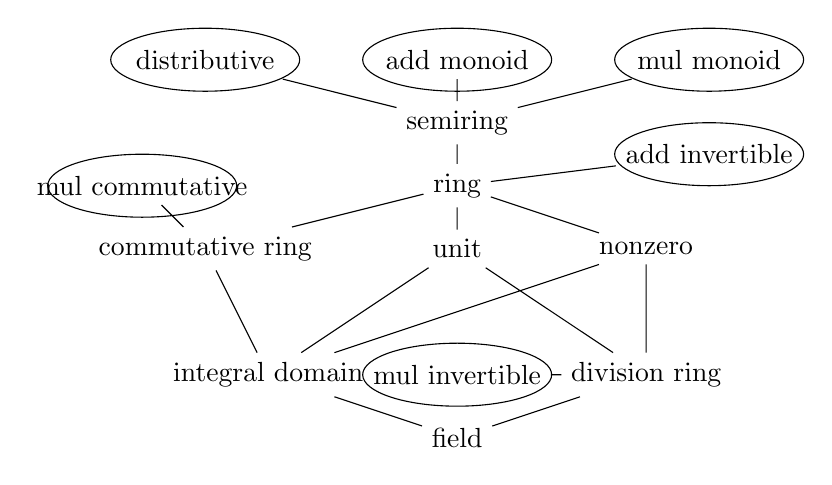
\begin{tikzpicture}[scale=0.8]
\draw (0, 1) node (semiring) {semiring}
      (0, 0) node (ring) {ring}
      (-4, -1) node (commu-ring) {commutative ring}
      (0, -1) node (unit) {unit}
      (3, -1) node (zero-factor) {nonzero}
      (-3, -3) node (integral-domain) {integral domain}
      (3, -3) node (division-ring) {division ring}
      (0, -4) node (field) {field};
\draw (0, 2) circle[x radius = 1.5cm, y radius = 0.5cm] node (add-monoid) {add monoid}
      (4, 2) circle[x radius = 1.5cm, y radius = 0.5cm] node (mul-monoid) {mul monoid}
      (-4, 2) circle[x radius = 1.5cm, y radius = 0.5cm] node (distribution-law) {distributive}
      (4, 0.5) circle[x radius = 1.5cm, y radius = 0.5cm] node (negate) {add invertible}
      (-5, 0) circle[x radius = 1.5cm, y radius = 0.5cm] node (mul-commu) {mul commutative}
      (0, -3) circle[x radius = 1.5cm, y radius = 0.5cm] node (mul-invert) {mul invertible};
\draw (distribution-law) to (semiring)
      (add-monoid) to (semiring)
      (mul-monoid) to (semiring)
      (semiring) to (ring)
      (negate) to (ring)
      (mul-commu) to (commu-ring)
      (ring) to (commu-ring)
      (ring) to (unit)
      (ring) to (zero-factor)
      (commu-ring) to (integral-domain)
      (unit) to (integral-domain)
      (zero-factor) to (integral-domain)
      (unit) to (division-ring)
      (zero-factor) to (division-ring)
      (integral-domain) to (field)
      (division-ring) to (field)
      (mul-invert) to (division-ring);
\end{tikzpicture}
\caption{semiring, ring, integral domain, and field}
\label{fig:ring}
\end{figure}

We omitted some important algebraic structure like subring, ideal, principal ideal domain, and Euclidean domain.

\section{Galois theory}

Galois theory provides connection between group and field. Using Galois theory, certain problems in field theory can be reduced to group theory, which is in some sense simpler and better understood. A field can contain infinite many elements with adding, subtracting, multiplying, and dividing. It's a complex mathematical object. Galois theory can simplify the problems in field to a corresponding problem in finite group with only one operation. This is the key idea of Galois theory.

Galois theory is famous for its difficulty and hard to understand. Compare to its original form, the modern Galois theory is no longer ambiguous, and much clearer and elegant. This is because more than two dozens of masters greatly developed and improved it in the past. The most important contributors are Jordan, Dedekind, and Emil Artin. Jordan and Dedekind first systematically developed Galois theory in France and Germany. The definition of Galois group we are using today was given by Dedekind. The modern form of Galois theory is made by Artin\cite{ZhangPu2013}. We adopted a gentle explanation that is friendly to new beginners\cite{Stillwell1994} in this short section. It's quite common that we can't understand it in the first time reading. It's always helpful to read the masters. Our life is not linear. I recommend way to revisit what we learned before, find more great books to read. Our understanding changes along the time, and there must be aha moment in the future.

\subsection{Field extension}
\index{field extension}

From the definition of field, we know that all rational numbers form a field $Q$. Let us consider a set of all the numbers in the form of $a + b\sqrt{2}$, where $a$ and $b$ are rational numbers\cite{Goodman2011}. Obviously, the set of rational numbers is a subset of it (just let $b = 0$). It's easy to verify that, for any two such numbers, the result of add, subtract, multiply, and divide is still in the form of $a + b \sqrt{2}$. Among them, divide takes more steps to verify. Given $x = \dfrac{1}{a + b\sqrt{2}}$, we can multiply both nominator and denominator by $a - b \sqrt{2}$ to have:

\[
\begin{array}{rl}
x & = \dfrac{a - b \sqrt{2}}{(a + b \sqrt{2})(a - b \sqrt{2})} \\[2ex]
  & = \dfrac{a - b \sqrt{2}}{a^2 - 2b^2}
\end{array}
\]

Let $p = a^2 - 2b^2$, then $x$ can be expressed as $(a/p) -(b/p)\sqrt{2}$. Thus we verified for divide operation as well. This set is really a field. We denote it as $Q[\sqrt{2}]$. Similarly, $Q[\sqrt{3}]$ is also a field. They are both example of field extension concept.

\begin{definition}
If field $E$ contains field $F$, then $E$ is \textbf{field extension} of $F$, denoted as $F \subseteq E$ or $E/F$.
\end{definition}

For example, real numbers is the field extension of rational numbers, $Q[\sqrt{2}]$ is the field extension of rational number field $Q$. Basically, for field $F$, if $\alpha \in F$, but $\sqrt{\alpha} \not\in F$, then $F_1 = F[\sqrt{\alpha}]$ is also a field. We can keep extending the field with this method. If $\beta \in F_1$, but $\sqrt{\beta} \not\in F_1$, then:

\[
\begin{array}{rl}
F_2 & = F_1[\sqrt{\beta}] \\
    & = F[\sqrt{\alpha}][\sqrt{\beta}] \\
    & = F[\sqrt{\alpha}, \sqrt{\beta}]
\end{array}
\]

All numbers like $a + b \sqrt{\beta}$ where $a, b \in F_1$ form a higher level field extension. Starting from rational numbers, we can obtain a series of field extensions $Q \subset F_1 \subset F_2 ... \subset F_n$.

Why does field extension matter? For example, equation $x^2 - 2 = 0$ can not be solved in the field of rational number (there are not any rational numbers satisfy this equation), however, if we extend from the rational number field, there are pair of solutions in the $Q[\sqrt{2}]$, which are $x = \pm \sqrt{2}$. Here is another example, for equation $x^4 - 5x^2 + 6 = 0$, there is no rational number solution, but there two solutions in field extension $Q[\sqrt{2}]$, which are $\pm \sqrt{2}$; if we extent the field one more step to $Q[\sqrt{2}, \sqrt{3}]$, we obtain the complete four solutions: $\pm \sqrt{2}$, and $\pm \sqrt{3}$. It leads to the important concept of \textbf{splitting field}.

\index{splitting field} \index{root field}
\begin{definition}
For equation $p(x) = 0$, the smallest field extension that contains all the roots is called the \textbf{splitting} field of $p(x)$. It's also called as root field.
\end{definition}

Thus the splitting field of equation $x^2 -2 = 0$ is $Q[\sqrt{2}]$. Why is it named as `splitting'? The polynomial $x^2-2$ can be decomposed in rational number field $Q$, however, in field extension $Q[\sqrt{2}]$ it can be {\em splits} to:
\[
(x + \sqrt{2}) (x - \sqrt{2})
\]

For a given polynomial equation, if we can start from the basic rational number field, with a series of field extension, reach to its splitting field, then this equation is radical solvable.

我们给出了平方根的例子,显然还有更加复杂的情况。3次方程可能要开3次方根,有些方程甚至还需要虚数单位$i$。从高中数学我们知道,最简单的方程$x^p-1=0$含有$p$个根$1, \zeta, \zeta^2, ..., \zeta^{p-1}$,其中$\zeta \neq 1$是单位圆上的一个复根。为了涵盖这些情况,我们需要更加严格地描述扩域。

\begin{figure}[htbp]
\centering
\begin{tikzpicture}[scale=3]
 \draw[step=.5cm, gray, very thin] (-1.2,-1.2) grid (1.2,1.2);
 \draw[->] (-1.25,0) -- (1.25,0) coordinate (x axis);
 \draw[->] (0,-1.25) -- (0,1.25) coordinate (y axis);
 \draw (0,0) circle (1cm);
 \draw[->, very thick] (0, 0) edge node[below=2pt,fill=white] {$\zeta^0 = \zeta^3 = 1$} (1, 0)
     (0, 0) edge node[above] {$\zeta = \dfrac{-1 + i\sqrt{3}}{2}$} (120:1cm)
     (0, 0) edge node[below] {$\zeta^2 = \dfrac{-1 - i\sqrt{3}}{2}$} (-120:1cm);
\end{tikzpicture}
\caption{单位根,$x^3 - 1 = 0$}
\label{fig:root-of-unity}
\end{figure}

如果$\alpha$的整数次方等于域$F$中的某个元素$b$,也就是说$\alpha^m = b \in F$,这样$\alpha$就可以写成$b$的根式形式$\alpha = \sqrt[m]{b}$。我们可以逐一用这样的一组根式进行扩域,从而得到$F[\alpha_1][\alpha_2]...[\alpha_k]$。如果每次扩张所用的$\alpha_i$都是根式,我们称扩域$F[\alpha_1, \alpha_2, ..., \alpha_k]$为$F$的根式扩域(radical extension)。设方程的根是$x_1, x_2, ..., x_n$(注意,这里我们没有说$x_i$一定是根式),如果其分裂域$E = Q[x_1, x_2, ..., x_n]$是根式扩域,我们说方程是根式可解的。

\begin{Exercise}
\Question{证明$Q[a, b] = Q[a][b]$,其中$Q[a, b]$是所有由$a, b$组成的表达式如$2ab, a + a^2b$等。}
\end{Exercise}

\subsection{自同构和伽罗瓦群}

到目前为止,我们的思路是从方程系数所在的有理数域开始,通过逐步根式扩域,向较高层次的分裂域前进。如何进一步化简难题,找到答案呢?伽罗瓦在此进行逆向思维。他转而去考虑方程根之间的对称性。例如方程$x^2 - 2 = 0$有一对根$\pm \sqrt{2}$。显然用$-\sqrt{2}$去代替$\sqrt{2}$,方程仍然成立。除此之外,将等式$\sqrt{2}^2 + \sqrt{2} + 1 = 3 + \sqrt{2}$中的$\sqrt{2}$替换成$-\sqrt{2}$也是成立的。也就是说,这对根$\pm \sqrt{2}$,对于关系$\alpha^2 + \alpha + 1 = 3\alpha$是对称的。进一步说,对于任何仅仅对$\sqrt{2}$进行乘法和加法的表达式,这对根都可以进行互换。今天我们知道,描述对称的最有力武器是群。具体说是置换群(如果记不清了,请回过头去再看一下\ref{symmetric group})。于是伽罗瓦引入了域上的自同构概念,将扩域和群联系了起来。

我们还是用$Q[\sqrt{2}]$举例子。如果我们定义一个从$Q[\sqrt{2}]$到$Q[\sqrt{2}]$的函数$f: Q[\sqrt{2}] \to Q[\sqrt{2}]$。它的具体定义为:
\[
f(a + b \sqrt{2}) = a - b \sqrt{2}
\]

则$f$就是一个域上的自同构。

\index{自同构}
\begin{definition}
\textbf{域的自同构}(Field Automorphism)是一个可逆函数$f$,它满足$f(x + y) = f(x) + f(y)$,$f(ax) = f(a) f(x)$,$f(1/x) = 1/f(x)$。
\end{definition}

我们可以验证,前面那个例子$f(a + b \sqrt{2}) = a - b \sqrt{2}$满足这三个条件。域的自同构背后的思想是,我们可以重新调换域中的元素,而完全不影响域的结构。

\begin{definition}
$F$-自同构:进一步,如果$E$是$F$的扩域,并且在域$E$的自同构$f$的基础上还满足一条额外的性质:对$F$中的任何元素$x$都有$f(x) = x$,则称为$E$上的$F$-自同构。
\end{definition}

这样就非常精确地定义了根的对称性。$F$-自同构对$F$中的所有元素都原样保持不动,而仅仅调换扩域$E$中新元素。对域中的元素进行调换恰好是置换(permutation)的思想,置换后保持不变恰好是对称的概念。对于$Q[\sqrt{2}]$这个例子,只有两个$Q$-自同构:一个是恒等变换$g(x) = x$,另外一个就是我们前面定义的$f$。

现在我们把目前得到的结果用例子$p(x) = x^2 - 2$总结一下:

\begin{enumerate}
\item $p(x)$的分裂域是$Q[\sqrt{2}]$;
\item $p(x)$的$Q$-自同构代表了根的对称性,它包含两个变换:$f(a + b\sqrt{2}) = a - b\sqrt{2}$和$g(x) = x$。
\end{enumerate}

但是仅仅扩展到分裂域并不能保证对所有的根完全对称。例如$x^4 - 5x + 6 = 0$的分裂域是$Q[\sqrt{2}, \sqrt{3}]$,虽然我们有能够调换$\pm \sqrt{2}$的自同构$f$,但是不存在能够调换$\sqrt{2}$和$\sqrt{3}$的自同构。否则根据自同构的定义$f(x) = x$,如果$f(\sqrt{2}) = \sqrt{3}$,则$f(\sqrt{2})^2 = \sqrt{3}^2$,即$\sqrt{2} = \sqrt{3}$。这显然是错误的。另外,考虑根式扩域$Q[x_1, ..., x_n, \sqrt{x_1}]$,它包含$x_1$的平方根,但是不含$x_2$的平方根。因此不存在能够调换$x_1$和$x_2$的自同构。为了恢复对称性,我们可以继续把$\sqrt{x_2}, ..., \sqrt{x_n}$扩展到域里。

\begin{theorem}
对于每个$Q[x_1, ..., x_n]$的根式扩域$E$,都存在一个更大的根式扩域$E \subseteq \overline{E}$,使得所有$x_1, ..., x_n$的置换都有自同构$\sigma$。
\end{theorem}

至此,我们已经把扩域和自同构联系了起来。如果把所有的自同构做成一个集合,这些自同构间的二元运算是复合(composite)变换,恒等变换是单位元,我们就得到了一个群。这个群被称作伽罗瓦群。

\index{伽罗瓦群}
\begin{definition}
\textbf{伽罗瓦群}:对于$F$的扩域$E$,我们有一组$E$的$F$-自同构的集合$G$。对任意$G$中的两个$F$-自同构$f, g$,定义二元运算$(f \cdot g)(x) = f(g(x))$。我们称$G$为扩域$E/F$的伽罗瓦群。记为$Gal(E/F)$。
\end{definition}

我们还是用$p(x) = x^2 - 2$举例。伽罗瓦群$G = Gal(p) = \{f, g\}$,包含两个元素,一个是$f(a + b\sqrt{2}) = a - b\sqrt{2}$,另一个是$g(x) = x$。其中单位元是$g$。我们来验证是否有$f \cdot f = g$:

\[
\begin{array}{rll}
(f \cdot f)(a + b\sqrt{2}) & = f(f(a + b\sqrt{2})) & \text{群运算的定义} \\
  & = f(a - b\sqrt{2}) & \text{对内层括号用$f$的定义} \\
  & = a + b\sqrt{2} & \text{再次用$f$的定义} \\
  & = g(a + b\sqrt{2}) & \text{恒等变换$g$的定义}
\end{array}
\]

这说明$G$的确是一个群,并且在同构的意义下等同于二阶循环群,它也同构于二阶对称群$S_2$。这个群可以写成$\{f, f^2\}$,这是因为$f^2 = f \cdot f = 1$,是群的单位元。也可写成置换群的形式$\{(1), (1\ 2)\}$,其中(1)是保持两个根不变,(1 2)是对调两个根。

\begin{Exercise}
\Question{试证明:对于有理数系数的任何多项式$p(x)$,若$E/Q$是扩域,$f$是$E$上的$Q$-自同构,则有$f(p(x)) = p(f(x))$。}
\Question{考虑复数,多项式$p(x) = x^4-1$的分裂域是什么?它的$Q$-自同构中有哪些变换?}
\Question{尝试写出二次方程$x^2 - bx + c = 0$的伽罗瓦群。}
\Question{证明,如果$p$是素数,则方程$x^p - 1$的伽罗瓦群是$q-1$阶的循环群$C_{q-1}$。}
\end{Exercise}

\subsection{伽罗瓦基本定理}
\index{伽罗瓦基本定理}

现在我们进入了伽罗瓦理论的核心部分了。从方程系数所在的域$F$开始,我们可以进行一系列扩域一直到达分裂域$F \subset F_1 \subset F_2 ... \subset E$。对应的伽罗瓦群为$Gal(E/F)$。伽罗瓦发现,这个群的所有子群和这些中间域$F_1, F_2, ...$之间存在着反序的一一对应。

\begin{theorem}
\textbf{伽罗瓦基本定理}:令$E/F$为扩域\footnote{严格说,要求是伽罗瓦扩张,我们这里略去了伽罗瓦扩张的定义。},$G$是对应的伽罗瓦群。这个群的子群和中间域之间存在一一对应。若$F \subset L \subset E$,有$Gal(E/L) = H$,则$H$是$Gal(E/F)$的子群。
\end{theorem}

之所以说是反序,是因为,随着域的扩张,对应的群是减小的。扩张的起点是域$F$,此时对应的群是完整的伽罗瓦群$G = Gal(E/F)$;扩张的终点是分裂域$E$,此时的群只有一个元素,就是恒等变换$\{1\}$。扩张的中间域$L$,对应的群是$H = Gal(E/L)$,它是子群,有$Gal(E/L) \subset Gal(E/F)$。并且如果$H$是正规子群(如果记不清了,可回去看一下\ref{normal-subgroup}),则它的商群$G/H = Gal(L/F)$。

我们举一个具体的例子\cite{MArtin}(490页)。考虑方程$x^4 - 8x^2 + 15 = 0$,它也可以表示成$(x^2 - 3)(x^2 - 5) = 0$。它的系数域是有理数域$Q$,方程的分裂域是$E = Q[\sqrt{3}, \sqrt{5}]$。它的伽罗瓦群$Gal(E/Q)$的阶是4,同构于一个4阶循环群。可以找到3个中间扩域分别是$Q[\sqrt{3}]$, $Q[\sqrt{5}]$和$Q[\sqrt{15}]$,这3个中间扩域对应的子群的阶都是2。而方程的伽罗瓦群,也就是4阶循环群只有一个2阶子群。除此之外,它不再有其它非平凡子群了。根据伽罗瓦基本定理,我们知道,除了那3个中间扩域之外,再也没有其它中间扩域了。换个角度看,分裂域上的任何元素都可以表示为$\alpha = a + b\sqrt{3} + c\sqrt{5} + d\sqrt{15}$,其中$a, b, c, d$是有理数;对于3个中间扩域上的任何元素,$b, c, d$中至少有两个为0。

\begin{figure}[htbp]
\centering
\begin{tikzpicture}[scale=0.8]
\draw (-3, 3) node (Q3-5) {$Q[\sqrt{3}, \sqrt{5}]$}
      (-5, 0) node (Q5) {$Q[\sqrt{5}]$}
      (-3, 0) node (Q15) {$Q[\sqrt{15}]$}
      (-1, 0) node (Q3) {$Q[\sqrt{3}]$}
      (-3, -3) node (Q) {$Q$};
\draw (3, 3) node (G1) {$\{1\}$}
      (1, 0) node (G3) {$\{1, f\}$}
      (3, 0) node (G15) {$\{1, (f \cdot g)\}$}
      (5, 0) node (G5) {$\{1, g\}$}
      (3, -3) node (G) {$\{1, f, g, (f \cdot g)\}$};
\draw[->] (Q3-5) edge node[midway, above] {伽罗瓦群} (G1)
      (G) edge node[midway, above] {对应到扩域} (Q)
      (Q3) edge node[midway] {扩域} (Q3-5)
      (Q15) edge (Q3-5)
      (Q5) edge (Q3-5)
      (Q) edge (Q3)
      (Q) edge (Q15)
      (Q) edge (Q5)
      (G1) edge node[midway] {子群} (G3)
      (G1) edge (G15)
      (G1) edge (G5)
      (G3) edge (G)
      (G15) edge (G)
      (G5) edge (G);
\end{tikzpicture}
\caption{伽罗瓦对应}
\label{fig:Galois-Correspondence}
\end{figure}

如图\ref{fig:Galois-Correspondence}所示,分裂域上的任意元可以写成如下形式:

\[
\begin{array}{rl}
\alpha &= (a + b\sqrt{3}) + (c + d\sqrt{3}) \sqrt {5} \\
       &= a + b\sqrt{3} + c\sqrt{5} + d\sqrt{15}
\end{array}
\]

其中$a, b, c, d$都是有理数。我们定义如下自同构:

变换$f$将$\sqrt{3}$反号:

\[
\begin{array}{rl}
f((a + b\sqrt{3}) + (c + d\sqrt{3}) \sqrt {5} & = (a - b\sqrt{3}) + (c - d\sqrt{3})\sqrt{5} \\
 & = a - b\sqrt{3} + c\sqrt{5} - d\sqrt{15}
\end{array}
\]

变换$g$将$\sqrt{5}$反号

\[
\begin{array}{rl}
g((a + b\sqrt{3}) + (c + d\sqrt{3}) \sqrt {5} & = (a + b\sqrt{3}) - (c + d\sqrt{3})\sqrt{5} \\
 & = a + b\sqrt{3} - c\sqrt{5} - d\sqrt{15}
\end{array}
\]

复合变换$f \cdot g$同时将$\sqrt{3}$和$\sqrt{5}$反号

\[
\begin{array}{rl}
(f \cdot g)((a + b\sqrt{3}) + (c + d\sqrt{3}) \sqrt {5} & = (a - b\sqrt{3}) - (c - d\sqrt{3})\sqrt{5} \\
 & = a - b\sqrt{3} - c\sqrt{5} + d\sqrt{15}
\end{array}
\]

%\begin{figure}[htbp]
\begin{wrapfigure}{R}{0.4\textwidth}
\centering

\begin{tikzpicture}[scale=0.7]
\filldraw[fill=gray, draw=gray] (-1, -2) rectangle (1, 2)
    (-2, -0.5) rectangle (2, 0.5);
\end{tikzpicture}
\captionsetup{labelformat=empty}
\caption{克莱因群的对称性。左右翻转,上下翻转,或者同时上下左右翻转都是对称的。}
\label{fig:Klein-four-group}
\end{wrapfigure}
%\end{figure}

再加上恒等变换1,基本域$Q$上的伽罗瓦群一共有4个元素:$G = \{1, f, g, (f \cdot g)\}$。这个群同构于克莱因群,而克莱因群相当于是两个2阶循环群的积。它共有5个子群,每个都对应着一个扩域:

\begin{itemize}
\item 只含有单位元$\{1\}$的子群,对应于分裂域$Q[\sqrt{3}, \sqrt{5}]$;
\item $G$自身,对应于有理数域$Q$;
\item 二阶子群$\{1, f\}$,对应于扩域$Q[\sqrt{5}]$,$f$只反转$\sqrt{3}$而固定$\sqrt{5}$不变;
\item 二阶子群$\{1, g\}$,对应于扩域$Q[\sqrt{3}]$,$f$只反转$\sqrt{5}$而固定$\sqrt{3}$不变;
\item 二阶子群$\{1, (f \cdot g)\}$,对应于扩域$Q[\sqrt{15}]$,$(f \cdot g)$同时反转$\sqrt{5}$和$\sqrt{3}$,而固定$\sqrt{15}$不变。
\end{itemize}

我们也可以把这个方程的伽罗瓦群写成置换群的形式:$\{(1), (1 2), (3 4), (1 2)(3 4)\}$。其中置换(1)表示保持4个根都不变;(1 2)表示交换$\pm \sqrt{3}$这两个根;(3 4)表示交换$\pm \sqrt{5}$这两个根;(1 2)(3 4)表示同时交换这两对根。

通过伽罗瓦基本定理,我们已经成功地将方程在域上的问题,转换为对称群的问题了。接下来要做的就是最后一击,通过群揭示可解性的本质。

\subsection{可解性}

通过伽罗瓦对应,我们将根式扩域的结构和群的结构联系起来了。为了简化问题,我们增加一些额外的限制。首先,我们假设每次根式扩域$F[\alpha_i]$中加入的$\alpha_i$都是素数次方根。例如对$\sqrt[6]{\alpha}$,我们把它拆成$\sqrt{\alpha} = \beta$和$\sqrt[3]{\beta}$,然后分两次进行根式扩域。其次,如果$\alpha_i$是$p$次方根,若扩域$F[\alpha_1, ..., \alpha_{i-1}]$中不含有$p$次单位根,我们可以认为$F[\alpha_1, ..., \alpha_i]$中也不含有$p$次单位根。除非$\alpha_i$本身就是$p$次单位根。举个例子,假设要加入$\alpha = \sqrt[3]{2}$进行根式扩域,如果上一个域$F$中不含有如图\ref{fig:root-of-unity}中的$\zeta = \dfrac{-1 + i\sqrt{3}}{2}$,我们可以认为扩域$F[\sqrt[3]{2}]$中也不含有$\zeta$。除非$\alpha^3 = 1$即$\alpha$本身就等于$\zeta$。如果这一点不成立,我们可以在加入$\alpha_i$之前先用$\zeta$进行扩域,这样域$F[\alpha_1, ..., \alpha_{i-1}, \zeta]$中就包含了所有$p$次单位根:$1, \zeta, \zeta^2, ..., \zeta^{p-1}$。以上这两个对根式扩域的修改并不会改变最终扩域的结果$F[\alpha_1, ..., \alpha_k]$。

这样,任何根式扩域$F[\alpha_1, ..., \alpha_k]$都组成一系列递增的链条:

\[
F = F_0 \subseteq F_1 \subseteq F_2 \subseteq ... \subseteq F_k = F[\alpha_1, ..., \alpha_k]
\]

其中每个$F_i = F_{i-1}[\alpha_i]$,而$\alpha_i$是$F_{i-1}$中某个元素的素数次方根。并且满足上面关于单位根的条件。和这一系列扩域链对应的,是一系列递减的子群链:

\[
Gal(F_k/F_0) = G_0 \supseteq G_1 \supseteq ... \supseteq G_k = Gal(F_k/F_k) = \{1\}
\]

其中$G_i = Gal(F_k/F_i) = Gal(F_k/F_{i-1}[\alpha_i])$。每一步从$G_{i-1}$前进到它的子群$G_i$,都反应了向域$F$中扩张素数次方根$\alpha_i$。用群论的术语说,$G_i$是前一个群$G_{i-1}$的正规子群,而商群$G_{i-1}/G_i$是阿贝尔群(可交换的)。我们下面来证明这点。

\begin{theorem}
如果扩域$B \subseteq B[\alpha] \subseteq E$中,$\alpha^p \in B$,$p$是素数。并且满足上面的单位根的条件,则$Gal(E/B[\alpha])$是群$Gal(E/B)$的正规子群,并且商群
\[
Gal(E/B) / Gal(E/B[\alpha])
\]
是阿贝尔群。
\end{theorem}

\begin{mdframed}
这一段的证明较难,一般的读者可以跳过框中的内容
\begin{proof}
我们要利用在\ref{normal-subgroup}中介绍的群同态定理来完成这一证明。我们要找到一个$Gal(E/B)$上的同态映射,它的核是$Gal(E/B[\alpha])$,它映射到一个阿贝尔群上。以$Gal(E/B[\alpha])$为核的映射显然限制在域$B[\alpha]$上,我们将这一映射记为$|_{B[\alpha]}$,根据伽罗瓦群的元素是自同构的定义:

\[
\sigma \in Gal(E/B[\alpha]) \iff \sigma|_{B[\alpha]} \text{是恒等变换}
\]

伽罗瓦群$Gal(E/B)$中所有这样的自同构$\sigma$满足同态映射的性质:

\[
\sigma'\sigma|_{B[\alpha]} = \sigma'|_{B[\alpha]}\sigma|_{B[\alpha]}
\]

由于$\sigma$固定所有$B$中的元素不变,所以$\sigma|_{B[\alpha]}$完全由$\sigma(\alpha)$决定。这里有两种情况。第一种情况是$\alpha$恰好等于$p$次单位根$\zeta$。此时:

\[
(\sigma(\alpha))^p = \sigma(\alpha^p) = \sigma(\zeta^p) = \sigma(1) = 1
\]

所以$\sigma(\alpha) = \zeta^i \in B[\alpha]$,这是因为每个$p$次单位根都是$\zeta^i$的形式。第二种情况下,$\alpha$不是$p$次单位根,此时:

\[
(\sigma(\alpha))^p = \sigma(\alpha^p) = \alpha^p
\]

根据根式扩域的规则,$\alpha^p$是$B$中的元素,所以$\sigma(\alpha) = \zeta^j\alpha$。其中$\zeta$是$p$次单位根,并且$\zeta \in B$。所以也有$\sigma(\alpha) \in B[\alpha]$。两种情况合并到一起,说明映射在每个$\sigma$下都是封闭的。

这就说明了$|_{B[\alpha]}$将伽罗瓦群$Gal(E/B)$映射到$Gal(E/B[\alpha])$。接下来我们要证明群$Gal(B[\alpha]/B)$是可交换的。我们仍然分两种情况来讨论:第一种情况$\alpha$是单位根,我们看到每个群中的元素,也就是自同构$\sigma_i = \sigma|_{B[\alpha]} \in Gal(B[\alpha]/B)$都可以写成$\sigma_i(\alpha) = \alpha^i$的形式,所以:

\[
\sigma_i\sigma_j(\alpha) = \sigma_i(\alpha^j) = \alpha^{ij} = \sigma_j\sigma_i(\alpha)
\]

第二种情况$\alpha$不是单位根,这样每个群中的元素,也就是自同构$\sigma_i$都可以写成$\sigma_i(\alpha) = \zeta^i\alpha$的形式,所以:

\[
\sigma_i\sigma_j(\alpha) = \sigma_i(\zeta^j\alpha) = \zeta^{i + j}\alpha = \sigma_j\sigma_i(\alpha)
\]

由于$\zeta \in B$,所以$\zeta$在自同构下固定不变。这样两种情况下,我们都证明了交换性。
\end{proof}
\end{mdframed}

这样回过头来看伽罗瓦群的子群链:

\[
Gal(F[\alpha_1, ..., \alpha_k]/F) = G_0 \supseteq G_1 \supseteq ... \supseteq G_k = \{1\}
\]

如果这链条中,每个群$G_i$都是上一个群$G_{i-1}$的正规子群,并且每个商群$G_{i-1}/G_i$都是可交换的,我们称伽罗瓦群$Gal(F[\alpha_1, ..., \alpha_k]/F)$是\textbf{可解的}。

现在我们来看一般的$n$次方程。

\[
x^n - a_1x^{n-1} + a_2x^{n-2}... \pm a_n = 0
\]

包含系数的基本域为$Q[a_1, ..., a_n]$。如果它的$n$个根(不一定为根式)是$x_1, ..., x_n$,即

\[
(x - x_1)...(x - x_n) = x^n - a_1x^{n-1} ... \pm a_n
\]

方程的根域为$Q[x_1, ..., x_n]$。如果无论怎样对基本域做根式扩域,都无法包含方程的根域,我们就说方程是无法用根式求解的。

\begin{theorem}
当$n \geq 5$时,$Q[a_1, ..., a_n]$的根式扩域不包含根域$Q[x_1, ..., x_n]$。
\end{theorem}

\begin{proof}
我们用反证法,假设某个根式扩域$E$包含根域$Q[x_1, ..., x_n]$,根据此前的定理,还存在更大个根式扩域$\overline{E} \supseteq E$,使得对应的伽罗瓦群$G_0 = Gal(\overline{E}/Q[a_1, ..., a_n])$包括所有根的置换的自同构。这样我们就可以构造一个子群的链条:

\[
G_0 \supseteq G_1 \supseteq ... \supseteq G_k = \{1\}
\]

每个$G_i$都是上一个群$G_{i-1}$的正规子群,并且商群$G_{i-1}/G_i$是可交换的。我们要证明这是不可能的。正规子群$G_i$是同态映射下$G_{i-1}$中的核,所以任意$G_{i-1}$中的两个自同构$\sigma, \tau$都有:

\[
\sigma^{-1}\tau^{-1}\sigma\tau \in G_{i}
\]

当$n$大于等于5时,$G_0$包含所有根的置换,同构于对称群$S_n$,它必然包含3循环的置换$(a\ b\ c)$。假设$G_{i-1}$中也包含3循环置换,我们有:

\[
(a\ b\ c) = (d\ a\ c)^{-1}(c\ e\ b)^{-1}(d\ a\ c)(c\ e\ b) \in G_i
\]

这说明$G_i$也包含3循环置换。根据数学归纳法,子群链条中所有的群都包含3循环置换。但这是不可能的,因为最后一个群是$\{1\}$,它不含3循环置换。
\end{proof}

\begin{figure}[htbp]
%\begin{wrapfigure}{R}{0.3\textwidth}
 \centering
 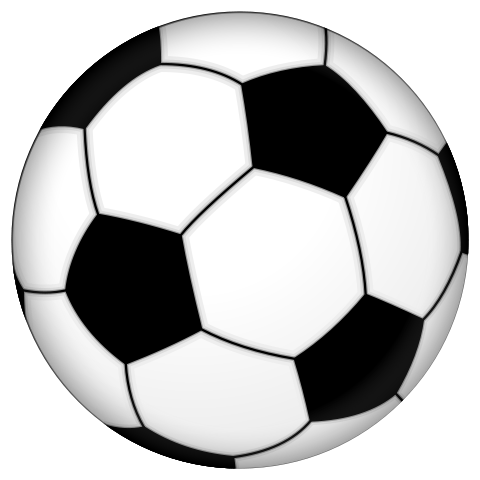
\includegraphics[scale=0.3]{img/Soccer-ball.eps}
 \captionsetup{labelformat=empty}
 \caption{对称群$S_5$是交错群$A_5$与二阶循环群的积。可以描述一个足球的对称}
 \label{fig:S5}
%\end{wrapfigure}
\end{figure}

这样我们就证明了一般5次方程是不能用根式解的。我们也可以从另一个角度做出解释。对称群$S_5$有120个元素,它的唯一正规子群是$A_5$,其中$A_5$叫做交错群,有60个元素。$A_5$的唯一正规子群是$\{1\}$。这一子群链是$S_5 \supset A_5 \supset \{1\}$。但是商群$A_5/\{1\}$不是阿贝尔群(不可交换)。因此它不是可解群。这样它对应的一般5次方程不是根式可解的。

一般4次方程,对称群$S_4$的正规子群是$A_4$,交错群$A_4$有一个正规子群

\[
\{(1), (1 2)(3 4), (1 3)(2 4), (1 4)(2 3)\}
\]

而这个群和克莱因群同构,所以是可解的。

对于三次方程,对称群$S_3$的正规子群$A_3$,交错群$A_3$同构于3阶循环群。所以也是可解的。

\begin{figure}[htbp]
  \centering
  \subcaptionbox{交错群$A_3$相当于3阶循环群}[0.3\linewidth]{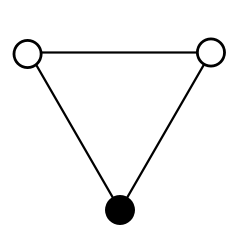
\includegraphics[scale=0.25]{img/C3.eps}} \quad
  \subcaptionbox{对称群$S_3$,其上部为$A_3$}[0.3\linewidth]{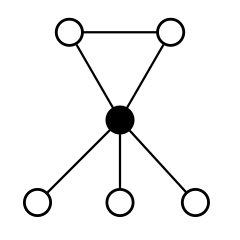
\includegraphics[scale=0.25]{img/S3.eps}}
  \subcaptionbox{交错群$A_4$}[0.3\linewidth]{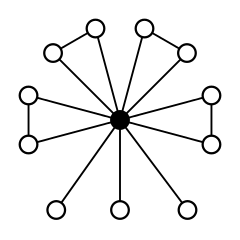
\includegraphics[scale=0.25]{img/A4.eps}}
  \caption{对称群和交错群,黑点是单位元,循环用闭环表示}
  \label{fig:group-graph}
\end{figure}

至此我们简单介绍了伽罗瓦理论。伽罗瓦理论是抽象代数中的强大工具,它可以解决很多问题,如证明代数基本定理、证明当年高斯用尺规作图画出的正17边形是可行的。证明无法用尺规作图完成古希腊三大作图问题——圆化方、三分角、倍立方等等。我们希望读者能通过这一章,领略到抽象思维的深邃和优美。

\begin{Exercise}
\Question{考虑5次方程$x^5 - 1 = 0$,它是根式可解的。它的伽罗瓦群和对应的子群链是什么?}
\end{Exercise}

\section{扩展阅读}

对于抽象代数的基本概念,张禾瑞先生的《近世代数基础》\cite{ZhangHeRui1978}是本入门的教材。这本书不到200页,提纲挈领地减少了群、环、域的基本概念。阿姆斯特朗的《群与对称》\cite{Armstrong1988}同样也是小薄本,对于对称性的讲解是其特色。迈克尔$\cdot$阿廷的《代数》是一本广泛使用的教材,最后一章讲解了伽罗瓦理论。爱德华兹的《伽罗瓦理论》,以历史的发展为主要脉络,用古典的方法来讲述。并且还把伽罗瓦手稿的英文译文置于附录,使读者能了解当初是怎样一步一步解决的问题。章璞先生的《伽罗瓦理论:天才的激情》\cite{ZhangPu2013}则用现代的方法讲解伽罗瓦理论。埃米尔$\cdot$阿廷的《伽罗瓦理论》是这个领域中的经典,有李同孚先生翻译的中译本。韩雪涛的《好的数学》系列中有很多数学家的传记故事,生动有趣。

\ifx\wholebook\relax \else
\begin{thebibliography}{99}

\bibitem{HanXueTao16}
{\fontspec{\cnmainft}韩雪涛 ``数学悖论与三次数学危机''. 人民邮电出版社.} 2016, ISBN: 9787115430434

\bibitem{LiuXinyu2017}
{\fontspec{\cnmainft}刘新宇 ``算法新解'' 人民邮电出版社.} 2017, ISBN: 9787115440358

\bibitem{HanXueTao2009}
{\fontspec{\cnmainft}韩雪涛 ``好的数学——“下金蛋”的数学问题''. 湖南科学技术出版社.} 2009, ISBN: 9787535756725

\bibitem{HanXueTao2012}
{\fontspec{\cnmainft}韩雪涛 ``好的数学——方程的故事''. 湖南科学技术出版社.} 2012, ISBN: 9787535770066

\bibitem{Wiki-Galois-theory}
Wikipedia ``Galois theory''. \url{https://en.wikipedia.org/wiki/Galois_theory}

\bibitem{Wiki-Galois}
Wikipedia ``Évariste Galois''. \url{https://en.wikipedia.org/wiki/Évariste_Galois}

\bibitem{Galois-1832}
Anita R Singh. ``The Last Mathematical Testament of Galois'' Resonance Oct 1999. pp93-100.

\bibitem{Liouville-1846}
Sawilowsky, Shlomo S. and Cuzzocrea, John L. (2005) ``Joseph Liouville’s `Mathematical Works Of Évariste Galois','' Journal of Modern Applied Statistical Methods: Vol. 5 : Iss. 2 , Article 32. DOI: 10.22237/jmasm/1162355460

\bibitem{StepanovRose15}
Alexander A. Stepanov, Daniel E. Rose ``From Mathematics to Generic Programming''. Addison-Wesley Professional; 1 edition (November 17, 2014) ISBN-13: 978-0321942043

\bibitem{Wiki-Rubik-Cube-group}
Wikipedia ``魔方群''. \url{https://en.wikipedia.org/wiki/Rubik's_Cube_group}

\bibitem{ZhangHeRui1978}
张禾瑞 ``近世代数基础''. 高等教育出版社. 1978, ISBN: 9787040012224

\bibitem{Armstrong1988}
M.A. Armstrong ``群与对称(影印版)''. Springer. 1988. ISBN: 0387966757.

\bibitem{Wiki-Lagrange}
Wikipedia ``约瑟夫$\cdot$拉格朗日''. \url{https://en.wikipedia.org/wiki/Joseph-Louis_Lagrange}

\bibitem{Wiki-FLT-proof}
Wikipedia ``费马小定理的证明''. \url{https://en.wikipedia.org/wiki/Proofs_of_Fermat's_little_theorem}

\bibitem{Wiki-Euler}
Wikipedia ``莱昂哈德$\cdot$欧拉''. \url{https://en.wikipedia.org/wiki/Leonhard_Euler}

\bibitem{Wiki-Carmichael-number}
Wikipedia ``卡米歇尔数''. \url{https://en.wikipedia.org/wiki/Carmichael_number}

\bibitem{Algorithms-DPV}
Sanjoy Dsgupta, Christos Papadimitriou, Umesh Vazirani. 钱枫 邹恒明 注释. ``算法概论(注释版)''. 机械工业出版社. 2009年1月. ISBN: 9787111253617

\bibitem{Wiki-Miller-Rabin}
Wikipedia ``米勒——拉宾素数检验''. \url{https://en.wikipedia.org/wiki/Miller-Rabin_primality_test}

\bibitem{Wiki-Noether}
Wikipedia ``埃米$\cdot$诺特''. \url{https://en.wikipedia.org/wiki/Emmy_Noether}

\bibitem{ZhangPu2013}
章璞. ``伽罗瓦理论:天才的激情''. 高等教育出版社. 2013年5月. ISBN: 9787040372526

\bibitem{Stillwell1994}
John Stillwell. ``Galois Theory for Beginners''. The American Mathematical Monthly, Vol. 101, No. 1 (Jan., 1994), pp. 22-2

\bibitem{Goodman2011}
Dan Goodman. ``An Introduction to Galois Theory''. \url{https://nrich.maths.org/1422}

\bibitem{MArtin}
Michael Artin. ``代数(英文版,第二版)''. 机械工业出版社. 2011年12月. ISBN: 9787111367017

\end{thebibliography}

\expandafter\enddocument
%\end{document}

\fi
